%%%%%%%%%%%%%%%%%%%%%%%%%%%%%%%%%%%%%%%%%%%%%%%%%%%%%%%%%%%%%%%%%%%%%%
% Lớp 12 | Ứng dụng đạo hàm để khảo sát hàm số | Đường tiệm cận
% Dạng 2D1?4-4: Toán thực tế ứng dụng tiệm cận
% Số câu: 12  (sinh tự động bởi tach_cau.py; từ nay thầy sửa trực tiếp file này)
%%%%%%%%%%%%%%%%%%%%%%%%%%%%%%%%%%%%%%%%%%%%%%%%%%%%%%%%%%%%%%%%%%%%%%

%%%%%%%%%%%%%%%% ĐÚNG/SAI %%%%%%%%%%%%%%%%

% nguồn: Phan1_Lop_12_Dai_so_Chuong_1
\begin{ex}%[2D1V4-4]%[ma:5333bab5]
	Cho hàm số $y=\dfrac{x^2-3x+6}{x-1}$ có  đồ thị $(C)$.
	 \choiceTF
		{\True Hàm số có đạo hàm $y'=\dfrac{x^2-2x-3}{\left(x-1\right)^2}$} 
		{Hàm số  có tập xác định $\mathscr{D}=\mathbb{R}\backslash\{-1\}$}
		{Các khoảng nghịch biến của hàm số  chứa $5$ số nguyên}
		{Gọi  $I$ tâm đối xứng của đồ thị $(C)$. Tiếp tuyến của đồ thị tại điểm có hoành độ $x=2$ cắt hai đường tiệm cận tại $A$, $B$. Diện tích tam giác $IAB$ bằng $12$}
	 \loigiai{
		\begin{itemchoice}
			\itemch Ta  có
			\begin{eqnarray*}
				 y'&=&\dfrac{\left(x^2-3x+6\right)'(x-1)-\left(x^2-3x+6\right)(x-1)'}{(x-1)^2} \\
				&=&\dfrac{(2x-3)(x-1)-(x^2-3x+6) \cdot 1}{\left(x-1\right)^2}\\ 
				&=&\dfrac{x^2-2x-3}{\left(x-1\right)^2}. 
			\end{eqnarray*}
			\itemch  Tập xác định của hàm số là $\mathscr{D}=\mathbb{R}\backslash\{1\}$.
			\itemch Ta có $y'=0 \Leftrightarrow x^2-2x-3 = 0 \Leftrightarrow \hoac{&x=-1 \\&x=3.}$ \\ 
			Bảng xét  dấu
			\begin{center}
				
\begin{tikzpicture}[scale=.75,transform shape]
					\tkzTabInit[nocadre=false,lgt=1.2,espcl=2.5,deltacl=0.6]{$x$ /1,$f’(x)$  /1}
						{$-\infty$,$-1$,$1$,$3$,$+\infty$} 
					\tkzTabLine{,+,0,-,d,-,0,+,} 
				\end{tikzpicture}
			\end{center}
			Hàm số nghịch biến  trên khoảng $(-1;1)$ và $(1;3)$ chứa các số nguyên là $0$; $2$.
			 \itemch Ta có
			\[\lim\limits_{x \rightarrow 1^+} y= \lim\limits_{x \rightarrow 1^+} \dfrac{x^2-3x+6}{x-1} =  +\infty.\]
			\[\lim\limits_{x \rightarrow 1^-} y=  \lim\limits_{x \rightarrow 1^-} \dfrac{x^2-3x+6}{x-1} = -\infty.\]
			$\Rightarrow x=1$ là đường tiệm cận đứng của đồ thị hàm số. 
			Ta  có
			\[y=\dfrac{x^2-3x+6}{x-1}=\dfrac{(x-1)^2 -(x-1)  +4}{x-1}=x-2+\dfrac{4}{x-1}.\]
			$\Rightarrow y=x-2$ là đường  tiệm cận xiên của đồ thị hàm số. \\
			Tâm đối xứng $I$ của đồ thị $(C)$ là giao điểm của hai đường tiệm cận. \\ 
			 $\Rightarrow I(1;-1)$. \\
			Ta có $y'(2) = -3$; $y(2) =  4$. \\
			Phương trình tiếp tuyến của đồ thị tại điểm  có hoành độ $x=2$ là
			\begin{eqnarray*}
				&&y-4=-3 \cdot (x-2)\\ 
				&\Leftrightarrow&y=-3x+10. 
			\end{eqnarray*}
			\begin{itemize}
				\item Tiếp tuyến  giao với đường tiệm cận đứng $x=1$ tại điểm $A(1;7)$.
				\item Tiếp tuyến giao với đường tiệm  cận xiên tại điểm $B(3;1)$.
			\end{itemize}
			 Ta có $IA=8$, $IB=2\sqrt{2}$, $AB=2\sqrt{10}$ \\
			Nửa chu vi tam giác $IAB$ là  $p=4+\sqrt{2}+\sqrt{10}$. \\
			Diện tích tam giác $IAB$  là
			\begin{eqnarray*}
				S&=&\sqrt{(4+\sqrt{2}+\sqrt{10})(4+\sqrt{2}+\sqrt{10}-8)(4+\sqrt{2}+\sqrt{10}-2\sqrt{2})(4+\sqrt{2}+\sqrt{10}-2\sqrt{10})} \\ 
				&=& 8. 
			\end{eqnarray*}
		\end{itemchoice}
	 }
\end{ex}

% nguồn: Phan1_Lop_12_Dai_so_Chuong_1
\begin{ex}%[2D1V4-4]%[ma:cd49f953]
	Một bể bơi chứa $5\,000$ lít nước tinh khiết. Người ta  bơm vào bể đó nước muối có nồng độ $30$ gam muối cho mỗi lít nước với tốc độ $25$ lít/phút.
	 \choiceTF
		{\True Sau $t$ phút khối lượng muối trong bể là $750t$ (gam)} 
		{Nồng độ muối trong bể sau $t$ phút (tính bằng tỉ số của khối  lượng muối trong bể và thể tích nước trong bể, đơn vị: gam/lít) là $f(t)=\dfrac{30t}{200-t}$}
		{\True Xem $y=f(t)$ là một hàm số xác định trên nửa khoảng $[0;+\infty)$, tiệm cận ngang của đồ thị hàm số  đó có phương trình là $y = 30$}
		{\True Khi $t$ ngày càng lớn thì  nồng độ muối trong bể sẽ tiến gần đến mức $30$ (gam/lít)}
	\loigiai{ 
		\begin{itemchoice}
			\itemch Sau $t$ phút, khối lượng muối trong bể  là
			\[ 
			25\cdot 30\cdot  t=750t \text{ (gam)}
			 \]
			\itemch Thể tích của lượng nước  trong bể là $5\,000+25t$ (lít).\\
			Vậy nồng độ muối sau $t$  phút là
			 \[
			 f(t)=\dfrac{750t}{5\,000+25t}=\dfrac{30t}{200+t}\,\text{ (gam/lít)}.
			 \]
			 \itemch
			 Ta có\\
			$\lim\limits_{t\to +\infty}f(t)=\lim\limits_{t \to +\infty}\dfrac{30t}{200+t}=\lim\limits_{t\to  +\infty}\left(30-\dfrac{6\,000}{200+t}\right)=30$.\\
			Vậy  đường thẳng $y=30$ là tiệm cận ngang của đồ thị hàm số $f(t)$.
			\begin{center}
				\begin{tikzpicture}[scale=.1,xscale=0.1,font=\footnotesize,line join=round,line cap=round,>=stealth]
					\draw[->] (-.5,0)--(0,0) node[below  right]{$O$}--(500,0) node[below]{$x$};
					\draw[->] (0,-1)  --(0,34) node[right]{$y$};
					\draw[blue]  [domain=0:500,samples=100]
						plot  (\x,{(30*(\x))/((\x)+200)});
					\draw[fill]  (0,0) circle (1pt);
					 \foreach \y/\g in {30/180}
					\draw[fill] (0,\y) circle (1pt)  node [shift={(\g:.3)}] {$\y$};
					\draw[red]  (-.1,30)--(500,30);
				\end{tikzpicture}
			\end{center}
			 \itemch
			Ta có đồ thị hàm số $y=f(t)$ nhận đường thẳng $y=30$ làm đường tiệm cận  ngang, tức là khi $t$ càng lớn thì nồng độ muối trong bể sẽ tiến gần đến mức $30$ (gam/lít). Lúc đó, nồng độ muối trong bể sẽ gần như bằng nồng độ nước muối bơm vào bể.
		\end{itemchoice}
	} 
\end{ex}


%%%%%%%%%%%%%%%% TRẢ LỜI NGẮN %%%%%%%%%%%%%%%%

% nguồn: Phan2_Lop_12_Dai_so_Chuong_1
\begin{bt}%[2D1H4-4]%[ma:bfaea089]
	Tại một công ty sản xuất đồ chơi an toàn cho trẻ em, công ty phải chi $34\,567$ USD để thiết lập dây chuyền sản xuất ban đầu. Sau đó, cứ sản xuất được một sản phẩm đồ chơi $X$, công ty phải trả $8$ USD  cho nguyên liệu ban đầu và nhân công. Gọi $x$ ($x \ge 1$) là số đồ chơi $X$ mà công ty đã sản xuất và $C(x)$ (đơn vị: USD) là tổng số tiền bao gồm cả chi phí ban đầu mà công ty phải chi trả khi sản xuất $x$ đồ chơi $X$. Khi đó chi phí trung bình cho mỗi sản phẩm đồ chơi $X$ là hàm số $\overline{C}(x)=\dfrac{C(x)}{x}$ xác định trên $[1;+\infty)$. Khi số đồ chơi sản xuất tăng lên thì chi phí trung bình cho mỗi sản phẩm đồ chơi $X$ giảm xuống nhưng không xuống dưới mức tối thiểu là bao nhiêu USD?
	\shortans{8} 
	 \loigiai{
		Ta có $C(x)  = 34\,567 + 8x$.\\
		Khi đó $\overline{C}(x) =  \dfrac{C(x)}{x} = \dfrac{34\,567 + 8x}{x} = 8 + \dfrac{34\,567}{x}$.\\
		Ta có $\lim\limits_{x \to +\infty} \overline{C}(x) =  \lim\limits_{x \to +\infty} \left(8 + \dfrac{34\,567}{x} \right) = 8$.\\
		Mà $\overline{C}(x)$ là hàm nghịch biến trên $[1;+\infty)$ nên chi phí  trung bình cho mỗi sản phẩm đồ chơi $X$ giảm xuống thấp nhất và không dưới $8$ USD.
	} 
\end{bt}

% nguồn: Phan2_Lop_12_Dai_so_Chuong_1
\begin{bt}%[2D1H4-4]%[ma:8fcb64d2]
	Số lượng sản phẩm bán được của một công ty trong $x$ (tháng) được  tính theo công thức $S(x)=200\left(5-\dfrac{9}{2+x}\right)$, trong đó $x \ge 1$. Số lượng sản phẩm lớn nhất mà công ty có thể bán được trong $x$ tháng là
	\shortans{1000} 
	 \loigiai{
		Số lượng sản phẩm bán được lớn nhất của công ty  là tiệm cận ngang của hàm số $S(x)$. \\
		Ta có $\lim\limits_{x  \to +\infty} y = \lim\limits_{x \to +\infty} 200\left(5-\dfrac{9}{2+x}\right)=1\,000$.\\
		 Vậy đường tiệm cận ngang của đồ thị hàm số $S(x)$ là $y=1\,000$.
	} 
\end{bt}

% nguồn: Phan2_Lop_12_Dai_so_Chuong_1
\begin{bt}%[2D1H4-4]%[ma:fdb9ead0]
	Một bể chứa $5\,000$ lít nước tinh khiết. Người ta bơm vào bể đó nước muối có nồng độ $30$ gam muối cho mỗi lít nước với tốc độ $25$ lít/phút. Nồng độ muối trong bể được tính bởi công thức $f(t) = \dfrac{30t}{200+t}$ ($t$ là thời gian nước chảy vào bể (phút)). Nồng độ muối lớn nhất mà bể có  thể đạt được là bao nhiêu gam/lít?
	 \shortans{30}
	\loigiai{ 
		Nồng độ muối lớn nhất mà bể có thể  đạt được là tiệm cận ngang của đồ thị hàm số. \\
		Ta  có
		$\lim\limits_{t  \to +\infty} f(t) = \lim\limits_{t \to +\infty} \dfrac{30t}{200+t} = \lim\limits_{t \to +\infty} \left(30 - \dfrac{6000}{200+t}\right) = 30$. \\
		Vậy nồng độ  muối lớn nhất của bể là $30$ gam/lit.
	} 
\end{bt}

% nguồn: Phan2_Lop_12_Dai_so_Chuong_1
\begin{bt}%[2D1V4-4]%[ma:1695c4d5]
	Một công ty sản xuất máy tính đã xác định được rằng, tính trung bình một nhân viên có thể lắp ráp được $N(x)=\dfrac{50 x}{x+4}(x \geq 0)$ bộ phận mỗi ngày sau $x$ ngày đào tạo. Xem $y=N(x)$ là một hàm  số xác định trên $[0;+\infty)$, khi số ngày đào tạo tăng lên, hãy tính số bộ phận một nhân viên lắp ráp tối đa không vượt quá bao nhiêu?
	 \shortans{50}
	 \loigiai{
		Ta có $\displaystyle\lim  _{x \rightarrow+\infty} N(x)=\displaystyle\lim _{x \rightarrow+\infty} \frac{50 x}{x+4}=\displaystyle\lim _{x \rightarrow+\infty} \frac{50}{1+\frac{4}{x}}=50$.
		Vậy một nhân viên lắp ráp tối đa không  vượt quá $50$ bộ phận máy tính.
	} 
\end{bt}

% nguồn: Phan2_Lop_12_Dai_so_Chuong_1
\begin{bt}%[2D1V4-4]%[ma:1be55739]
	Nồng độ thuốc trong máu của một bệnh nhân sau khi tiêm $t$ giây là $P(t) \left(\dfrac{mg}{m l}\right)$. Với $P(t)$ cho bởi công thức $P(t)=\sqrt{0{,}09 t^{2}+0{,}018t+0{,}05}-0{,}3t$. Nồng độ thuốc tồn dư, tức nồng độ thuốc vẫn còn trong cơ thể bệnh  nhân trong dài hạn khi tiêm là bao nhiêu?
	 \shortans{0,03}
	\loigiai{ 
		Do đề bài cho  nồng độ thuốc trong cơ thể bệnh nhân trong dài hạn nên $t \to +\infty$.\\
		Ta  có
		\begin{eqnarray*}
			\lim\limits_{t \to +\infty} P(t)&=&\lim\limits_{t \to +\infty}\left(\sqrt{0{,}09 t^{2}+0{,}018 t+0{,}05}-0{,}3 t\right)  \\
			&=&\lim\limits_{t  \to+\infty} \dfrac{0{,}09 t^{2}+0{,}018 t+0{,}05-(0{,}3 t)^{2}}{\sqrt{0{,}09 t^{2}+0{,}018 t+0{,}05}+0{,}3 t} \\
			&=&\lim\limits_{t \to+\infty} \dfrac{0{,}018 t+0{,}05}{\sqrt{0{,}09 t^{2}+0{,}018 t+0{,}05}+0{,}3 t}  \\
			&=&\lim\limits_{t \to +\infty}  \dfrac{t\left(0{,}018+\dfrac{0{,}05}{t}\right)}{t\left(\sqrt{0{,}09+\dfrac{0{,}018}{t}+\dfrac{0{,}05}{t^{2}}}+0{,}3\right)} \\
			&=&\lim\limits_{t  \to +\infty} \dfrac{0{,}018+\dfrac{0{,}05}{t}}{\sqrt{0{,}09+\dfrac{0{,}018}{t}+\dfrac{0{,}05}{t^{2}}}+0{,}3}=\dfrac{0{,}018}{\sqrt{0{,}09}+0{,}3}=0{,}03.
		\end{eqnarray*}
		Vậy nồng độ thuốc tồn dư trong cơ thể bệnh nhân  là $0{,}03\left(\dfrac{\mathrm{mg}}{\mathrm{ml}}\right)$.
	} 
\end{bt}

% nguồn: Phan2_Lop_12_Dai_so_Chuong_1
\begin{bt}%[2D1V4-4]%[ma:c103a57d]
	Giả sử doanh số $f(t)$ (tính bằng số sản phẩm) của một sản phẩm mới (trong vòng một số năm nhất định) tuân theo quy luật logistic được mô  hình hoá bằng hàm số $f(t) = \dfrac{5000}{1 + 5e^{-t}}, (t \ge 0)$, trong đó thời gian $t$ được tính bằng năm kể từ khi phát hành sản phẩm mới. Khi đó đạo hàm $f'(t)$ là biểu thị tốc độ bán hàng. Hỏi sau khi phát hành bao~nhiêu năm thì tốc độ bán hàng là lớn nhất? (làm tròn kết quả đến hàng phần chục).
	\shortans{1,6} 
	\loigiai{ 
		Xét hàm  số:
		$$ f(t) = \dfrac{5000}{1+5e^{-t}}, (t \ge 0)  $$
		Vì đạo hàm $f'(t)$ là biểu thị tốc độ bán hàng nên để biết sau khi phát hành bao~nhiêu năm thì tốc độ bán hàng là lớn nhất ta  tìm GTLN của hàm số:
		$$ f'(t) = \dfrac{25000e^{-t}}{(1+5e^{-t})^2}, (t \ge 0)  $$
		$$  f''(t) = \dfrac{25000e^{-t}(5e^{-t}-1)}{(1+5e^{-t})^3} $$
		$$ f''(t)=0 \Leftrightarrow \dfrac{25000e^{-t}(5e^{-t}-1)}{(1+5e^{-t})^3} = 0 \Leftrightarrow  5e^{-t}-1=0 \Leftrightarrow e^{-t}=\dfrac{1}{5} \Leftrightarrow t=\ln 5 $$
		Bảng  biến thiên:
		\begin{center}
			
\begin{tikzpicture}[scale=0.7,transform shape]
				 \tkzTabInit[nocadre,espcl=5]
					{$t$/1,$f'(t)$/1,$f  (t)$/3}
					{$0$,$ \ln 5 $,$ +\infty  $}
				\tkzTabLine{,+,0,-,} 
				 \tkzTabVar{-/,+/$\max$,-/}
			\end{tikzpicture}
		\end{center}
		 Hàm số $f'(t)$ đạt GTLN khi $t=\ln 5 \approx 1,6$. \\
		Vậy  sau khi phát hành 1,6 năm thì tốc độ bán hàng là lớn nhất.
	 }
\end{bt}

% nguồn: Phan2_Lop_12_Dai_so_Chuong_1
\begin{bt}%[2D1V4-4]%[ma:8bdcac8c]
	Chi phí xuất bản $x$ cuốn tạp chí (bao gồm: lương cán bộ, công nhân viên, giấy in...) được cho bởi $C(x) = x^2 - 2000x + 10^8$ đồng. Chi phí phát hành cho mỗi cuốn là 4 nghìn đồng ($4000$ đồng). $M(x) = \dfrac{T(x)}{x}$ với $T(x)$ là tổng chi phí (xuất bản và phát hành) cho $x$  cuốn tạp chí, được gọi là chi phí trung bình cho một cuốn tạp chí khi xuất bản $x$ cuốn. Khi số lượng cuốn tạp chí phát hành cực lớn thì chi phí trung bình cho mỗi cuốn tạp chí $M(x)$ sẽ tiệm cận với đường thẳng có phương trình dạng $y=ax+b$. Tính $P=68a+3b+800$.
	 \shortans{6868}
	 \loigiai{
		Theo giả thiết, ta có: \\ 
		$T(x)=C(x)+4000x = x^2 - 2000x + 10^8 + 4000x = x^2 + 2000x + 10^8$ (đồng). \\ 
		$M(x)  = \dfrac{T(x)}{x} = \dfrac{x^2 + 2000x + 10^8}{x} = x + \dfrac{10^8}{x}+2000 $. \\
		$\lim\limits_{x \to +\infty} [M(x) - (x+2000)] =  \lim\limits_{x \to +\infty} \left[x + 2000 + \dfrac{10^8}{x} - (x+2000) \right] = \lim\limits_{x \to +\infty} \dfrac{10^8}{x} = 0$. \\
		Khi đó đồ thị hàm số $M(x) =  x + 2000 + \dfrac{10^8}{x}$ có 1 tiệm cận xiên là $y = x+2000$. \\
		Khi số lượng cuốn tạp chí phát hành  cực lớn thì chi phí trung bình cho mỗi cuốn tạp chí $M(x)$ sẽ tiệm cận với đường thẳng $y=x+2000$. \\
		Suy ra $\heva{&a=1  \\ &b=2000.}$ \\
		Vậy $P = 68a +  3b + 800 = 68 \cdot 1 + 3 \cdot 2000 + 800 = 6868$.
	 }
\end{bt}

% nguồn: Phan2_Lop_12_Dai_so_Chuong_1
\begin{bt}%[2D1V4-4]%[ma:996158d8]
	Một bể chứa $1\,000$ lít nước tinh khiết. Người ta bơm vào bể đó nước muối có nồng độ $15$ gam muối cho mỗi lít nước  với tốc độ $20$ lít/phút. Biết rằng nồng độ muối trong bể sau $t$ phút (tính bằng tỉ số của khối lượng muối trong bể và thể tích nước trong bể, đơn vị: gam/lít) là một hàm số $f(t)$, thời gian $t$ tính bằng phút. Phương trình tiệm cận ngang của đồ thị hàm số $f(t)$ bằng là $y=a$, $(a \in \mathbb{R})$. Tìm $a$.
	 \shortans{15}
	 \loigiai{
		Sau $t$ phút,  ta có khối lượng muối trong bể là $20 \cdot 15t = 300t$ (gam). \\
		Thế tích của lượng nước trong  bể sau $t$ phút là $1\,000+20t$ (lít). \\
		Do đó nồng độ muối sau  $t$ phút là $f(t) = \dfrac{300t}{1\,000+20t} = \dfrac{30t}{100+2t}$ (gam/lít). \\
		Ta có $\lim\limits_{t \to +\infty} f(t) = \lim\limits_{t \to +\infty} \dfrac{30t}{100+2t} = \dfrac{30}{2} = 15$ nên đồ thị  hàm số $y = f(t)$ có phương trình tiệm cận ngang là $y=15$. \\
		 Vậy $a=15$.
	 }
\end{bt}

% nguồn: Phan2_Lop_12_Dai_so_Chuong_1
\begin{bt}%[2D1V4-4]%[ma:bfc97649]
	Một cơ sở sản xuất tính toán rằng số sản phẩm trung bình mà một nhân viên làm được mỗi ngày là $f(x)=\dfrac{100 x}{x+10}$ với $x$ là số ngày kinh nghiệm làm việc $(x \geq 0)$. Xem $y=f(x)$ là một hàm số xác định trên $[0;+\infty)$. Khi số ngày kinh nghiệm làm việc tăng lên thì số sản  phẩm trung bình tối đa mà một nhân viên có thể làm được trong một ngày là bao nhiêu?
	 \shortans{99}
	 \loigiai{
		Ta có: $f(x)=\dfrac{100 x}{x+10}=100-\dfrac{1000}{x+10}<100$ và $\displaystyle\lim _{x \rightarrow+\infty} f(x)=100$.\\ Nên số sản phẩm tối đa mà một nhân viên  làm được trong một ngày là không quá 99 sản phẩm.
		Ta có $f(x)=99  \Leftrightarrow \dfrac{100 x}{x+10}=99 \Leftrightarrow x=990$.
		Vậy khi số ngày kinh  nghiệm làm việc tăng lên thì số sản phẩm trung bình tối đa mà một nhân viên có thể làm được trong một ngày là $99$ .
	} 
\end{bt}

% nguồn: Phan2_Lop_12_Dai_so_Chuong_1
\begin{bt}%[2D1V4-4]%[ma:c91cf04a]
	Để loại bỏ $x$\,\% chất gây  ô nhiễm không khí từ khí thải của một nhà máy, người ta ước tính chi phí cần bỏ ra là $C(x) = \dfrac{300x}{100 - x}$ (triệu đồng), $0 \le x < 100$. Tìm số đường tiệm cận đứng của đồ thị hàm số $y = C(x)$.
	 \shortans{1}
	\loigiai{ 
		Tập xác định  $\mathscr{D} = [0;100)$. \\
		Xét hàm số $y = C(x) = \dfrac{300x}{100-x}$, $0 \leq x <  100$. \\
		Ta có  $y' = \dfrac{30\,000}{(100-x)^2} > 0$, với mọi $x \in [0;100)$. \\
		Do đó hàm số luôn đồng biến trên  nửa khoảng $[0;100)$. \\
		Vì $\lim\limits_{x \to 100^-} C(x) = \lim\limits_{x \to 100^-} \dfrac{300x}{100-x} = +\infty$, nên đồ thị hàm số có tiệm cận  đứng là $x = 100$.
	 }
\end{bt}

% nguồn: 2026-11-16_12_2D1_TL_Ham_so (nhập 16/11/2026)
\begin{bt}%[2D1H4-4]%[ma:ad79ed70]
% nguon: Archive/SP_SauLuoi_2024-2025/SP_GHKI/2-TN-DS-TLN-TL-THPT-ChuyenLeKhiet-QuangNgai-GHKI-NH24-25.tex #342
%[KNTT - Lớp 12 - Kiểm tra giữa học kì 1 - THPT Liên Khiết-Quãng Ngãi]%[Ngô Tất Thành]
	Một công ty sản xuất đồ chơi $A$ phải chi $30\,000$ USD để thiết lập dây chuyền sản xuất ban đầu. Sau đó, cứ sản xuất được một sản phẩm đồ chơi $A$, công ty phải trả $4$ USD cho nguyên liệu thô và nhân công. Gọi $x \ (x \geq 1)$ là số đồ chơi mà công ty đã sản xuất và $T(x)$ (đơn vị USD) là tổng số tiền bao gồm cả chi phí ban đầu mà công ty phải trả khi sản xuất $x$ đồ chơi $A$. Người ta xác định chi phí trung bình cho mỗi sản phẩm đồ chơi $A$ là $M(x) = \dfrac{T(x)}{x}$. Khi $x$ đủ lớn $(x \to +\infty)$ thì chi phí trung bình cho mỗi sản phẩm đồ chơi $A$ gần nhất là bao nhiêu USD?
	\loigiai{ 
		Chi phí trung bình để sản xuất một sản phẩm $A$ là $M(x) = \dfrac{4x + 30\,000}{x}$. \\
		Ta có $\lim\limits_{x\to +\infty}M(x)=\lim\limits_{x\to +\infty}\dfrac{4x + 30\,000}{x}=4$. \\
		Vậy chi phí trung bình cho mỗi sản phẩm đồ chơi $A$ là gần $4$ USD.			
	}
\end{bt}

% nguồn: 2026-11-16_12_2D1_TL_Ham_so (nhập 16/11/2026)
\begin{bt}%[2D1N4-4]%[ma:7e262c28]
% nguon: Archive/2024/0. [LVH] BG - 12 New - 4in1-20240625T224301Z-001/0. [LVH] BG - 12 New - 4in1/2. [LVH] TEX SGK 12 NEW-20240418T074833Z-001/2. [LVH] TEX SGK 12 NEW/[LVH] SGK-12-KNTT/data/C1/12-SGK-KNTT-1-3.tex #1096

	Để loại bỏ $p\%$ một loài tảo độc khỏi một hồ nước, người ta ước tính chi phí bỏ ra là
	$$
	C(p)=\dfrac{45p}{100-p} \text { (triệu đồng), với } 0 \leq p<100.
	$$
	Tìm tiệm cận đứng của đồ thị hàm số $C(p)$ và nêu ý nghĩa thực tiễn của đường tiệm cận này.
	\loigiai{
		Ta có $\displaystyle\lim_{p\to 100^-}C(p)=\displaystyle\lim_{p\to 100^-}\dfrac{45p}{100-p}=+\infty$. \\
		Suy ra đồ thị hàm số có tiệm cận đứng là đường thẳng $p=100$.\\
		Ý nghĩa thực tiễn: Để loại bỏ hoàn toàn loài tảo độc trên thì chi phí vô cùng lớn (không thể thực hiện được).
	}
\end{bt}

% nguồn: 2026-11-16_12_2D1_TL_Ham_so (nhập 16/11/2026)
\begin{bt}%[2D1N4-4]%[ma:2b22e648]
% nguon: Archive/2024/TaiLieuGiangDay/1.HamSo/1. K12 - 4in1 - Hamso/ThubaiGoc/Bai4-Dang6.tex #2507
[SGK12-CTST, Mức độ 1]%[Bài giảng 12, Phạm Tiến Long]
Theo thuyết tương đối hẹp, khối lượng m (kg) của một hạt phụ thuộc vào tốc độ di chuyển $v(\mathrm{~km} / \mathrm{s})$ của nó trong hệ quy chiếu quán tính theo công thức $m(v)=\dfrac{m_0}{\sqrt{1-\dfrac{v^2}{c^2}}}$, trong đó $m_0$
là khối lượng nghỉ của hạt, $c=300000 \mathrm{~km} / \mathrm{s}$ là tốc độ ánh sáng. 
	Tìm tiệm cận của đồ thị hàm số khối lượng hạt.
	\loigiai{
		Hàm số $y=m(v)=\dfrac{m_{0}}{\sqrt{1-\dfrac{v^{2}}{c^{2}}}}$ có tập xác định $\mathscr{D}=\left[0;c\right)$.\\
		Ta có $\lim\limits_{x \rightarrow c^-} \dfrac{m_{0}}{\sqrt{1-\dfrac{v^{2}}{c^{2}}}}=+\infty$.\\
		Vậy đồ thị hàm số có tiệm cận đứng là đường thẳng $x=c=300\,000$.	
	}
\end{bt}

% nguồn: 2026-11-16_12_2D1_TL_Ham_so (nhập 16/11/2026)
\begin{bt}%[2D1N4-4]%[ma:4f7919bb]
% nguon: Archive/2024/TaiLieuGiangDay/1.HamSo/1. K12 - 4in1 - Hamso/ThubaiGoc/Bai4-Dang6.tex #2511
[SGK12-CTST, Mức độ 1]%[Bài giảng 12, Phạm Tiến Long]
	Nồng độ oxygen trong hồ theo thời gian $t$ cho bởi công thức $y(t)=5-\dfrac{15t}{9t^{2}+1}$, với $y$ được tính theo mg/l và $t$ được tính theo giờ, $t \geq 0$. Tìm các đường tiệm cận của đồ thị hàm số $y(t)$. Từ đó, có nhận xét gì về nồng độ oxygen trong hồ khi thời gian $t$ trở nên rất lớn?
	\begin{flushright}
		%	(Theo: \href{www.researchgate.net/publication/264903978_Microrespirometric_characterization_of_activated_sludge_inhibition_by_copper_and_zinc}{www.researchgate.net/publication/264903978\_Microrespirometric\_characterization\_of\_activated\_sludge\_inhibition\_by\_copper\_and\_zinc})
		(\textit{Theo}: www.researchgate.net/publication/264903978\_Microrespirometric\_\\
		characterization\_of\_activated\_sludge\_inhibition\_by\_copper\_and\_zinc)
	\end{flushright}
	\loigiai{
		Hàm số $y(t)=5-\dfrac{15t}{9t^{2}+1}$ có tập xác định $\mathscr{D}=\mathbb{R}$.\\
		Ta có $\lim\limits_{x \rightarrow+\infty} \left(5-\dfrac{15t}{9t^{2}+1}\right)=5$.\\
		Vậy đồ thị hàm số có tiệm cận ngang là đường thẳng $y=5$.\\
		Khi thời gian $t$ trở nên rất lớn thì nồng độ oxygen trong hồ sẽ tiến dần về $5$ mg/l.
	}
\end{bt}

% nguồn: 2026-11-16_12_2D1_TL_Ham_so (nhập 16/11/2026)
\begin{bt}%[2D1N4-4]%[ma:ee2ba243]
% nguon: Archive/2024/TaiLieuGiangDay/1.HamSo/1. K12 - 4in1 - Hamso/ThubaiGoc/Bai4-Dang6.tex #2512
[SGK12-CKP, Mức độ 2]%[Bài giảng 12, Phạm Tiến Long]
	\immini{
		Tại một công ty sản xuất đồ chơi $A$, công ty phải chi $50\,000$ USD để thiết lập dây chuyền sản xuất ban đầu. Sau đó, cứ sản xuất được một sản phẩm đồ chơi $A$, công ty phải trả $5$ USD cho nguyên liệu thô và nhân công. Gọi $x$ ($x\geq 1$) là số đồ chơi $A$ mà công ty đã sản xuất và $T(x)$ (đơn vị USD) là tổng tiền bao gồm cả chi phí ban đầu mà công ty phải chi trả khi sản xuất $x$ đồ chơi $A$. Người ta xác định chi phí trung bình cho mỗi sản phẩm đồ chơi $A$ là $M(x)=\dfrac{T(x)}{x}$.
		\begin{enumerate}
			\item Xem $M(x)$ là hàm số theo $x$ xác định trên nửa khoảng $[1;+\infty)$, tìm tiệm cận ngang của đồ thị hàm số này.
			\item Nêu nhận xét về chi phí trung bình cho mỗi sản phẩm đồ chơi $A$ khi $x$ đủ lớn.
		\end{enumerate}
	}{
		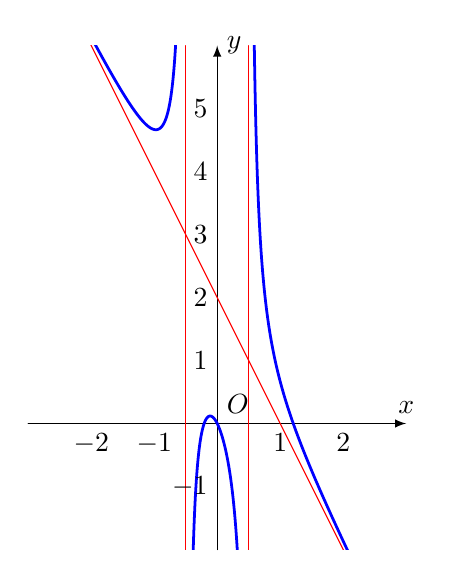
\begin{tikzpicture}[>=latex,line join=round, line cap=round, scale=0.8]
			\draw[->] (-3,0)--(3,0) node[above]{$x$};
			\draw[->] (0,-2)--(0,6) node[right]{$y$};
			\clip (-3,-2) rectangle (3,6);
			\draw[samples=200,smooth,blue,line width=1] plot[domain=-3:-0.51] (\x,{2-2*(\x)+2/(4*(\x)^2-1))});
			\draw[samples=200,smooth,blue,line width=1] plot[domain=-0.49:0.49] (\x,{2-2*(\x)+2/(4*(\x)^2-1))});
			\draw[samples=200,smooth,blue,line width=1] plot[domain=0.51:3] (\x,{2-2*(\x)+2/(4*(\x)^2-1))});
			\draw[samples=200,smooth,red] plot[domain=-3:3] (\x,{2-2*(\x)});
			\draw[red] (-0.5,-2)--(-0.5,6) (0.5,-2)--(0.5,6);
			\draw (0,0) node[above right]{$O$} (-2,0) node[below]{$-2$} (-1,0) node[below]{$-1$} (1,0) node[below]{$1$} (2,0) node[below]{$2$} (0,-1) node[left]{$-1$} (0,1) node[left]{$1$} (0,2) node[left]{$2$} (0,3) node[left]{$3$} (0,4) node[left]{$4$} (0,5) node[left]{$5$};
		\end{tikzpicture}
	}
	\loigiai{
		\begin{enumerate}
			\item Chi phí bỏ ra để sản xuất đồ chơi là $T(x)=50\,000+5x$ (USD).\\
			Chi phí trung bình cho mỗi sản phẩm là $M(x)=\dfrac{T(x)}{x}=\dfrac{50\,000+5x}{x}$ (với $x\geq 1$).\\
			Ta có $\lim\limits_{x\to \pm\infty}M(x)=5$. Suy ra đường thẳng $y=5$ là tiệm cận ngang của đồ thị.
			\item Khi số đồ chơi $A$ được sản xuất với số lượng $x$ đủ lớn thì chi phí trung bình tiệm cận với tổng của giá nguyên liệu thô và nhân công.
		\end{enumerate}
	}
\end{bt}

% nguồn: 2026-11-16_12_2D1_TL_Ham_so (nhập 16/11/2026)
\begin{bt}%[2D1C4-4]%[ma:83a7cec8]
% nguon: Archive/2024/San pham - To Latex Strong - Tex hoa Lop 12 moi - Dot 3 (Chuong 1 + 2 +3 + 4)/Data/Chuong 1/Canh dieu/To 3 - Dot 16 - Chuong 1 - Bai 3 - CD - De 2.tex #3584
%[Tổ 3 - Đợt 16 - Chương 1 - Bài 3 - Cánh Diều - Đề 2]%[Đình Nguyên]
	\immini{Người ta muốn làm một cái bể dạng hình hộp chữ nhật không nắp (như hình vẽ) có thể tích bằng $5$m$^3$. Chiều cao của bể là $10$dm, các kích thước khác là $x$m, $y$m với $x > 0$ và $y > 0$. Diện tích toàn phần của bể (không kể nắp) là hàm số $S(x)$ trên khoảng $(0;+\infty)$. Đường tiệm cận xiên của đồ thị hàm số $S(x)$ là đường thẳng $y=a x+b$. Tính giá trị của biểu thức $P=a^2+b^2$}
	{
		\begin{tikzpicture}[scale=1, font=\footnotesize, line join=round, line cap=round, >=stealth]
			\def\bc{4} \def\ba{2} \def\h{2} \def\gocB{35} 
			\coordinate[label=below left:$B$] (B) at (0,0);
			\coordinate[label=above left:$A$] (A) at (\gocB:\ba);
			\coordinate[label=below:$C$] (C) at (\bc,0);
			\coordinate[label=right:$D$] (D) at ($(C)-(B)+(A)$);
			\coordinate[label=above left:$A'$] (A') at ($(A)+(90:\h)$);
			\coordinate[label=left:$B'$] (B') at ($(B)-(A)+(A')$);
			\coordinate[label=below right:$C'$] (C') at ($(C)-(A)+(A')$);
			\coordinate[label=right:$D'$] (D') at ($(D)-(A)+(A')$);
			\draw (B')--(B)--(C)--(D)--(D')--(A')--(B')--(C')--(D') (C)--(C');
			\draw[dashed] (A')--(A)--(D) (A)--(B);
			%	\foreach \diem in {A,B,C,D,A',B',C',D'}	\fill (\diem)circle(1pt);
		\end{tikzpicture}
		
	}
	
	\loigiai{
		Do thể tích của bể là $1$m$^3$ nên $1\cdot x  y \Leftrightarrow xy=5$.\\
		Diện tích toàn phần của bể là $S(x)=xy+2x+2y=5+2x+\dfrac{10}{x}, \quad x>0$.\\
		Ta có $\lim\limits_{x \to+\infty}\left(S(x)-5-2 x\right)=\lim\limits_{x \to+\infty}\left(\dfrac{10}{x}\right)=0$.\\
		Suy ra đồ thị hàm số $S(x)$ có đường tiệm cận xiên là $y=2x+5$.\\
		Suy ra $a=2$; $b=5$.\\
		Vậy $P=a^2+b^2+2^2+5^2=29$.
	}
\end{bt}

% nguồn: 2026-11-16_12_2D1_TT_Ham_so (nhập 16/11/2026)
\begin{bt}%[2D1H4-4]%[ma:d439ddb4]
% nguon: Archive/SP_SauLuoi_2024-2025/SP_HKI/2-TN-DS-TLN-THPT-NgoQuyen-HKI-HCM-NH23-24.tex #162
%[Dự án đề KT Toán khối 12 HKI NH23-24-Trịnh Văn Cảnh]%[THPT Ngô Quyền - TPHCM]
	Tổng chi phí để sản xuất $x$ sản phẩm của một xí nghiệp được tính theo công thức
	\[T(x)=2 x^2+x+25 \text { (nghìn đồng). }\]
	Chi phí trung bình của $1$ sản phẩm khi sản xuất được $x$ sản phẩm là $C(x)$. Xem $y=C(x)$ là một hàm số xác định trên khoảng $(0 ;+\infty)$, tiệm cận xiên của đồ thị hàm số này là đường thẳng $y=ax+b$. Giá trị của $a+b$ là bao nhiêu?
	\shortans{$3$}
	\loigiai{Chi phí trung bình của 1 sản phẩm khi sản xuất được $x$ sản phẩm là:
		\[C(x)=\dfrac{T(x)}{x}=\dfrac{2 x^2+x+25}{x}=2x+1+\dfrac{25}{x}.\]
		Ta thấy $\lim\limits_{x \to +\infty} [C(x) - (2x+1)]=\lim\limits_{x \to +\infty} \dfrac{25}{x}=0$.\\
		Do đó đường thẳng $y=2x+1$ là tiệm cận xiên của đồ thị hàm số $y=C(x)$.\\
		Suy ra $a=2$ và $b=1$.\\
		Vậy giá trị $a+b=2+1=3$.
	}
\end{bt}

% nguồn: 2026-11-16_12_2D1_TT_Ham_so (nhập 16/11/2026)
\begin{bt}%[2D1V4-4]%[ma:9d7a252e]
% nguon: Archive/SP_SauLuoi_2024-2025/SP_GHKI/2-TN-DS-TLN-THPT-BuiThiXuan-GHKI-NH24-25.tex #182
%[Lớp 12 - Ôn tập giữa học kì 1 năm 24-25 - Bùi Thị Xuân TP HCM]%[Phạm Văn Long]
	Một công ty sản xuất máy tính đã xác định được rằng: tính trung bình một nhân viên có thể lắp ráp được $P(x)=\dfrac{500x}{4x+25}$ bộ phận mỗi ngày sau $x$ ngày được đào tạo, với $x \geq 0$. Xem $y=P(x)$ là một hàm số xác định trên $[0;+\infty)$ thì $y=a$ là đường tiệm cận ngang của đồ thị hàm số. Xác định giá trị $a$.
	\shortans{125}
	\loigiai{
	Ta có $\lim\limits_{x \to +\infty}\dfrac{500x}{4x+25}=125$ nên $y=125$ là đường tiệm cận ngang của đồ thị hàm số.\\ Vậy $a=125$.
	}
\end{bt}

% nguồn: 2026-11-16_12_2D1_TT_Ham_so (nhập 16/11/2026)
% nguồn: 2026-11-16_12_2D1_TT_Ham_so (nhập 16/11/2026)
\begin{bt}%[2D1V4-4]%[ma:6b7cc569]
% nguon: Archive/SP_SauLuoi_2024-2025/SP_GHKI/2-TL-TN-DS-THPT-Ly-Thuong-Kiet-GHKI-NH24-25.tex #249
%[Dự án đề kiểm tra Toán khối 12 GHKI NH24-25- Đợt 3 - Nhật Thiện]%[Trường THPT LÝ THƯỜNG KIỆT - HCM]
	Một công ty sản xuất đồ chơi ước tính chi phí để sản xuất $x$ (sản phẩm), $x>0$ là $C(x)=2x^2-x+25$ (nghìn đồng). Gọi $f(x)$ là chi phí trung bình sản xuất mỗi sản phẩm. Phương trình đường tiệm cận xiên của đồ thị hàm số $y=f(x)$ có dạng $y=ax+b$. Tính $T=b-a$.
	\shortans{-3}
	\loigiai{
	Chi phí trung bình sản xuất mỗi sản phẩm là $f(x)=\dfrac{C(x)}{x}=2x-1+\dfrac{25}{x}$.\\
	Ta có $\lim\limits_{x\to +\infty} \left[f(x)-(2x-1)\right]=\lim\limits_{x\to +\infty} \dfrac{25}{x}=0$.\\
	Suy ra $y=2x-1$ là tiệm cận xiên của đồ thị hàm số.\\
	Vậy $a=2$ và $b=-1$, do đó $T=b-a=-3$.
}
\end{bt}

% nguồn: 2026-11-16_12_2D1_TT_Ham_so (nhập 16/11/2026)
\begin{bt}%[2D1H4-4]%[ma:b79b3f96]
% nguon: Archive/SP_SauLuoi_2024-2025/SP_GHKI/2-TN-DS-TLN-THPT-NgoQuyen-HCM-GHKI-NH24-25.tex #267
%[Đề kiểm tra giữa HK 1, Năm học 2024-2025,Nguyễn Đức Lợi]%[THPT Ngô Quyền - TPHCM]
	Số dân của một thị trấn sau $t$  năm kể từ năm 1970 được ước tính bởi công thức $f(t) = \dfrac{20t+5}{t+2}$ ($f(t)$ được tính bằng nghìn người). Xem $y=f(t)$  là một hàm số xác định trên nửa khoảng $[0; +\infty)$. Đồ thị hàm số $y=f(t)$ có đường tiệm cận ngang là  $y=a$. Giá trị của $a$ là bao nhiêu?
	\shortans{20}
	\loigiai{
		Ta có $\lim \limits_{t \to +\infty} f(t) = \lim \limits_{t \to +\infty} \dfrac{20t + 5}{t + 2} =  \lim \limits_{t \to +\infty} \dfrac{20 + \dfrac{5}{t}}{1 + \dfrac{2}{t}} = \dfrac{20 + 0}{1 + 0} = 20$.\\
		Suy ra tiệm cận ngang của đồ thị hàm số $f(t)$ là đường thẳng $y = 20$.\\
		Vậy $a = 20$.
	}
\end{bt}

% nguồn: 2026-11-16_12_2D1_TT_Ham_so (nhập 16/11/2026)
\begin{bt}%[2D1H4-4]%[ma:137bb409]
% nguon: Archive/SP_SauLuoi_2024-2025/SP_GHKI/2-TN-DS-TLN-THPT-chuyenLeQuyDon-NinhThuan-GHKI-NH24-25.tex #332
%[CD - Lớp 12 - KT GHKI - Chuyên Lê Quý Đôn - Ninh Thuận]%[VU Ngoc Hao]
	Một công ty chuyên sản xuất đồ gia dụng ước tính chi phí để sản xuất $x$   sản phẩm là $C(x)=2x+250$ (triệu đồng), khi đó $G(x)=\dfrac{C(x)}{x}$  là chi phí sản xuất cho mỗi sản phẩm. Số lượng sản phẩm càng nhiều thì chi phí sản xuất mỗi sản phẩm càng nhỏ nhưng không thể thấp hơn $a$ (triệu đồng). Hãy tính giá trị $a$.
	\shortans{$2$}
	\loigiai{ 
	Ta có $G(x)=\dfrac{C(x)}{x}=\dfrac{2x+250}{x}$.\\
	$a=\lim\limits_{x\to+\infty}G(x)=\lim\limits_{x\to+\infty}\dfrac{2x+250}{x}=2$. }
	
\end{bt}

% nguồn: 2026-11-16_12_2D1_TT_Ham_so (nhập 16/11/2026)
% nguồn: 2026-11-16_12_2D1_TT_Ham_so (nhập 16/11/2026)
\begin{bt}%[2D1H4-4]%[ma:6213abe8]
% nguon: Archive/2024/San pham - To Latex Strong - Tex hoa Lop 12 moi - Dot 2 (Chuong 1 + 2 + 3)/San pham - To Latex Strong - Tex hoa Lop 12 moi - Dot 2 (Chuong 1 + 2 + 3)/Data/Chuong 1/Ket noi tri thuc/To 14 - Dot 16 - Chuong 1 - Bai 3 - KNTT - De 2.tex #762
%[Tổ 14 - Đợt 16 - Chương 1 - Bài 3 - KNTT]%[Lam Nguyen]
	Một mảnh vườn hình chữ nhật có diện tích bằng $100$ m$^2$. Biết chiều dài của mảnh vườn đó là $x$ (m), gọi chu vi của mảnh vườn là $P(x)$. Tìm số đường tiệm cận của đồ thị hàm số $P(x)$.
	\shortans{$2$}
	\loigiai{
		Ta có, chiều rộng của mảnh vườn là $\dfrac{100}{x}$.\\
		Chu vi của mảnh vườn là $P(x)=2\left(x+\dfrac{100}{x}\right)=2 x+\dfrac{200}{x}$.\\
		Mặt khác, ta có\\
		$\lim\limits_{x \to+\infty}P(x)=\lim\limits_{x \to+\infty}\left(2 x+\dfrac{200}{x}\right)=+\infty$.\\
		$\lim\limits_{x \to-\infty} P(x)=\lim\limits_{x \to-\infty}\left(2 x+\dfrac{200}{x}\right)=-\infty$. \\
		Vậy đồ thị hàm số $P(x)$ không có tiệm cận ngang.\\
		$\lim\limits_{x \to 0^-}P(x)=\lim\limits_{x \to 0^-}\left(2 x+\dfrac{200}{x}\right)=-\infty$.\\
		$\lim\limits_{x \to 0^+} P(x)=\lim\limits_{x \to 0^+}\left(2 x+\dfrac{200}{x}\right)=+\infty$.\\
		Vậy đồ thị hàm số $P(x)$ có tiệm cận đứng là $x=0$.\\\
		$\lim\limits_{x \to \pm \infty}\left[P(x)-2x\right]=\lim\limits_{x \to \pm \infty}\left(2 x+\dfrac{200}{x}-2 x\right)=0$ nên đồ thị hàm số $P(x)$ có tiệm cận xiên là $y=2 x$.}
\end{bt}

% nguồn: 2026-11-16_12_2D1_TT_Ham_so (nhập 16/11/2026)
\begin{bt}%[2D1V4-4]%[ma:ee8b7a52]
% nguon: Archive/2024/San pham - To Latex Strong - Tex hoa Lop 12 moi - Dot 2 (Chuong 1 + 2 + 3)/San pham - To Latex Strong - Tex hoa Lop 12 moi - Dot 2 (Chuong 1 + 2 + 3)/Data/Chuong 1/Ket noi tri thuc/To 14 - Dot 16 - Chuong 1 - Bai 3 - KNTT - De 2.tex #763
%[Tổ 14 - Đợt 16 - Chương 1 - Bài 3 - KNTT]%[Lam Nguyen]
	Chi phí xuất bản $x$ cuốn tạp chí (bao gồm: Lương cán bộ, công nhân viên, giấy in, $\ldots$) được cho bởi công thức $C(x)=0{,}001 x^2+3 x+1000$, $C(x)$ được tính theo đơn vị nghìn đồng. Chi phí phát hành cho mỗi cuốn là $4$ nghìn đồng. Tổng chi phí (xuất bản và phát hành) cho $x$ cuốn tạp chí là $T(x)$. Gọi $M(x)=\dfrac{T(x)}{x}$ được gọi là chi phí trung bình cho một cuốn tạp chí khi xuất bản $x$ cuốn. $a$ là số tiệm cận của đồ thị hàm số $M(x)$ và $b$ là số lượng tạp chí cần xuất bản sao cho chi phí trung bình là thấp nhất. Tính $b-10a$.
	\shortans{$980$}
	\loigiai{
		Tổng chi phí cho $x$ cuốn tạp chí là $T(x)=C(x)+4 \cdot x=0\text{,}001x^2+7 x+1000$.\\
		Ta có $M(x)=0\text{,}001 x+\dfrac{1000}{x}+7$ với $x=1{,}2, \ldots$\\
		Xét hàm số $y=M(x)$ trên khoảng $(0 ;+\infty)$.\\
		Ta có $\lim\limits_{x \to+\infty}\left[ M(x)-0\text{,}001 x-7\right]=0$;\\ $\lim\limits_{x \to-\infty}\left[ M(x)-0\text{,}001 x-7\right] =0$.\\
		Suy ra $y=0\text{,}001 x+7$ là tiệm cận xiên.\\
		Ta có $\lim\limits_{x \to 0^+}M(x)=+\infty$;  $\lim\limits_{x \to 0^-}M(x)=-\infty$.\\ Suy ra $x=0$ là tiệm cận đứng.\\
		Vậy $a=2$.\\
		Ta có $M(x)=0\text{,}001 x+\dfrac{1000}{x}+7$ với $x=1{,}2, \ldots$. Tìm GTNN của hàm số $M(x)$ trên $(0 ;+\infty)$.\\
		$M'(x)=0\text{,}001-\dfrac{1000}{x^2}=0 \Leftrightarrow x=1000$.\\
		Bảng biến thiên
		\begin{center}
		
\begin{tikzpicture}
		\tkzTabInit[espcl=2.5,lgt=1.5]
		{$x$/0.7,$M'(x)$/0.7,$M(x)$/2.1}
		{$0$,$1000$,$+\infty$}
		\tkzTabLine{,-,0,+}
		\tkzTabVar{+/,-/$9$,+/}
		\end{tikzpicture}
		\end{center}
		Suy ra $\min\limits_{(0 ;+\infty)} M(x)=M(1000)=9$.\\
		Vậy chi phí trung bình cho $x$ cuốn tạp chí thấp nhất khi $x=1000$, chi phí cho mỗi cuốn khi đó là $9$ nghìn đồng. Khi đó $b=1000$.\\
		Vậy $b-10a=1000-20=980$.}
\end{bt}

% nguồn: 2026-11-16_12_2D1_TT_Ham_so (nhập 16/11/2026)
\begin{bt}%[2D1V4-4]%[ma:1c363455]
% nguon: Archive/2024/San pham - To Latex Strong - Tex hoa Lop 12 moi - Dot 2 (Chuong 1 + 2 + 3)/San pham - To Latex Strong - Tex hoa Lop 12 moi - Dot 2 (Chuong 1 + 2 + 3)/Data/Chuong 1/Chan troi sang tao/To 26 - Dot 16 - Chuong 1 - Bai 3 - CTST - De 2.tex #803
%[Tổ 27 - Đợt 16 - Chương 1 - Bài 3 - CTST - Đề 2]%[Phùng Minh Phúc]
	Người ta thống kê được chi phí sửa chữa, vận hành máy móc trong một năm của một xưởng sản xuất được tính bởi công thức $f\left( x \right)=\dfrac{2\,000x-1\,500}{35x+5}$ (triệu đồng). Biết $x$ là số năm kể từ lúc máy móc vận hành lần đầu tiên, số năm càng nhiều thì chi phí càng cao. Khi số năm $x$ đủ lớn thì chi phí vận hành máy móc trong một năm gần với số nào? (làm tròn đến $1$ chữ số thập phân sau dấu phẩy).\\
	\shortans[oly]{57,1}
	\loigiai{
		Ta có: $\underset{x\to +\infty }{\mathop{\lim }}\,f\left( x \right)=\underset{x\to +\infty }{\mathop{\lim }}\,\dfrac{2\,000x-1\,500}{35x+5}=\dfrac{2\,000}{35}=\dfrac{400}{7}$.\\
		Do đó đồ thị hàm số $y=f\left( x \right)$ nhận đường thẳng $y=\dfrac{400}{7}$ làm tiệm cận ngang, tức là khi số năm $x$ càng lớn thì chi phí vận hành máy móc trong một năm càng tiến gần đến $\dfrac{400}{7}\approx 57{,}1$ (triệu đồng).
	}
\end{bt}

% nguồn: 2026-11-16_12_2D1_TT_Ham_so (nhập 16/11/2026)
\begin{bt}%[2D1V4-4]%[ma:71279ce1]
% nguon: Archive/2024/San pham - To Latex Strong - Tex hoa Lop 12 moi - Dot 2 (Chuong 1 + 2 + 3)/San pham - To Latex Strong - Tex hoa Lop 12 moi - Dot 2 (Chuong 1 + 2 + 3)/Data/Chuong 1/Chan troi sang tao/To 26 - Dot 16 - Chuong 1 - Bai 3 - CTST - De 2.tex #804
%[Tổ 27 - Đợt 16 - Chương 1 - Bài 3 - CTST - Đề 2]%[Phùng Minh Phúc]
	Để thiết kế một bể cá hình hộp chữ nhật có chiều cao là $80\,\mathrm{cm}$, thể tích là $12\,800\,\mathrm{cm^3}$. Người thợ dùng loại kính để sử dụng làm mặt bên có giá thành $70\,000\,\mathrm{VND/m^2}$ và loại kính đề làm mặt đáy có giá thành $100\,000\, \mathrm{VND/m^2}$. Gọi $x$ là chiều dài của đáy bể cá với $\left( x>0,\,\,x\,(\mathrm{m}) \right)$; $f\left( x \right)$ là hàm số xác định chi phí để hoàn thành bể cá. Có bao nhiêu đường tiệm cận của đồ thị hàm số $f\left( x \right)$.\\
	\shortans[oly]{2}
	\loigiai{
		Gọi $y$ là chiều rộng của đáy bể cá $\left( y>0,\,y\,(\mathrm{m}) \right)$.\\
		Ta có $0{,}8xy=0{,}0128\Rightarrow y=\dfrac{0{,}016}{x}\left( \mathrm{m} \right)$.\\
		Giá thành bể cá được xác định theo hàm số:\\
		$f\left( x \right)=2\cdot0{,}8\left( x+\dfrac{0{,}016}{x} \right)\cdot 70\,000+100\,000\cdot x\cdot\dfrac{0{,}016}{x}$ (VNĐ)\\
		$\Rightarrow f\left( x \right)=112\,000\left( x+\dfrac{0{,}016}{x} \right)+1\,600$(VNĐ)
		$\Rightarrow f\left( x \right)=112\,000x+1\,600+\dfrac{1\,792}{x}$(VNĐ).\\
		Ta có\\
		$\underset{x\to {{0}^{+}}}{\mathop{\lim }}\,f\left( x \right)=\underset{x\to {{0}^{+}}}{\mathop{\lim }}\,\left( 112\,000x+1\,600+\dfrac{1\,792}{x} \right)=+\infty $.\\
		$\underset{x\to +\infty }{\mathop{\lim }}\,\left[ f\left( x \right)-(112\,000x+1\,600) \right]=\underset{x\to +\infty }{\mathop{\lim }}\,\dfrac{1\,792}{x}=0$.\\
		Nên đồ thị hàm $f\left( x \right)$ có tiệm cận đứng là $x=0$; tiệm cận xiên là $y=112\,000x+1\,600$.\\
		Vậy có $2$ đường tiệm cận.
	}
\end{bt}

% nguồn: 2026-11-16_12_2D1_TT_Ham_so (nhập 16/11/2026)
\begin{bt}%[2D1H4-4]%[ma:1c803973]
% nguon: Archive/2024/San pham - To Latex Strong - Tex hoa Lop 12 moi - Dot 2 (Chuong 1 + 2 + 3)/San pham - To Latex Strong - Tex hoa Lop 12 moi - Dot 2 (Chuong 1 + 2 + 3)/Data/Chuong 1/Canh dieu/To 3 - Dot 16 - Chuong 1 - Bai 3 - CD - De 2 - GV khong nop bai.tex #870
%[Tổ 3 - Đợt 16 - Chương 1 - Bài 3 - Cánh Diều]%[Thơ Thơ] 
	Số lượng sản phẩm bán được của một cửa hàng quần áo trong $t$ (tháng) được cho bởi công thức: $S(t)=200\left(\dfrac{2}{3}-\dfrac{8}{2+t}\right)$ với $t \geq 1$. Xem $y=S(t)$ là một hàm số xác định trên nửa khoảng $[1 ;+\infty)$, biết rằng tiệm cận ngang của đồ thị hàm số có dạng $\dfrac{a}{b}, a, b \in \mathbb{N}^*,(a, b)=1$. Tính $P=a-2 b$.
	\shortans{$394$}
	\loigiai
	{Ta có : $\lim\limits _{x \rightarrow+\infty} S(t)=\lim\limits _{x \rightarrow+\infty} 200\left(\dfrac{2}{3}-\dfrac{8}{2+t}\right)=200 \cdot \dfrac{2}{3}=\dfrac{400}{3} \Rightarrow a=400 ; b=3$.\\
		Vậy $P=a-2 b=400-6=394$.
	}
\end{bt}

% nguồn: 2026-11-16_12_2D1_TT_Ham_so (nhập 16/11/2026)
\begin{bt}%[2D1H4-4]%[ma:78f8852d]
% nguon: Archive/2024/San pham - To Latex Strong - Tex hoa Lop 12 moi - Dot 2 (Chuong 1 + 2 + 3)/San pham - To Latex Strong - Tex hoa Lop 12 moi - Dot 2 (Chuong 1 + 2 + 3)/Data/Chuong 1/Canh dieu/To 3 - Dot 16 - Chuong 1 - Bai 3 - CD - De 2 - GV khong nop bai.tex #872
%[Tổ 3 - Đợt 16 - Chương 1 - Bài 3 - Cánh Diều]%[Thơ Thơ] 
	Từ một tấm tôn hình chữ nhật có các kích thước là $x$(m), $y$(m) với $x>1$; $y>1$ và diện tích bằng $4 \text{m}^2$. Người ta cắt bốn hình vuông bằng nhau ở bốn góc rồi gập thành một cái thùng dạng hình hộp chữ nhật không nắp (như hình vẽ) có chiều cao bằng $0{,}5$m. Thể tích của thùng là hàm số $V(x)$ trên khoảng $(1 ;+\infty)$. Đồ thị hàm số $y=\dfrac{1}{V(x)}$ có bao nhiêu đường tiệm cận đứng?
	\begin{center}
		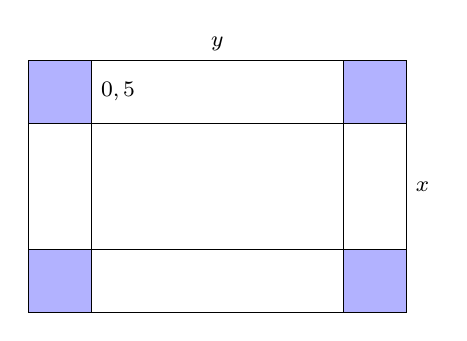
\begin{tikzpicture}[scale=0.8, font=\footnotesize, >=stealth]
			\coordinate (A) at (0,0);
			\coordinate (B) at (6,0);
			\coordinate (C) at (6,4);
			\coordinate (D) at (0,4);
			\fill[blue!30](A)--(1,0)--(1,1)--(0,1)--cycle;
			\fill[blue!30](B)--(5,0)--(5,1)--(6,1)--cycle;
			\fill[blue!30](C)--(5,4)--(5,3)--(6,3)--cycle;
			\fill[blue!30](D)--(1,4)--(1,3)--(0,3)--cycle;
			\draw (A) -- (B) -- (C) -- (D) -- (A);
			\draw (1,0) -- (1,4) (5,0) -- (5,4) (0,1) -- (6,1) (0,3) -- (6,3);
			\coordinate[label=above:{$y$}] (c) at (3,4);
			\coordinate[label=right:{$x$}] (b) at (6,2);
			\coordinate[label=right:{$0,5$}] (d) at (1,3.5);
		\end{tikzpicture}
		\hspace{1cm}
		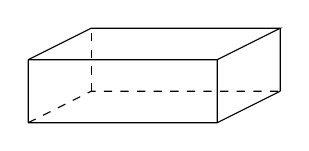
\begin{tikzpicture}[scale=0.8, font=\footnotesize, >=stealth]
			\coordinate (A) at (0,0);
			\coordinate (B) at (3,0);
			\coordinate (C) at (4,0.5);
			\coordinate (D) at (1,0.5);
			\coordinate (E) at (0,1);
			\coordinate (F) at (3,1);
			\coordinate (G) at (4,1.5);
			\coordinate (H) at (1,1.5);
			\draw (A) -- (B)--(C) (A)--(E) (B)--(F) (C)--(G);
			\draw (E) -- (F) -- (G) -- (H) -- (E);
			\draw[dashed] (A)--(D)--(C);
			\draw[dashed] (D)--(H);
		\end{tikzpicture}
	\end{center}
	\shortans{$2$}
	\loigiai
	{Do tấm tôn có diện tích bằng $4 \text{m}^2$ nên $x y=4 \Leftrightarrow y=\dfrac{4}{x}$.\\
		Thùng có chiều cao là $0{,}5$m và các kích thước còn lại của thùng là : $x-1$ và $y-1$.\\
		Thể tích của thùng là $$V(x)=0{,}5(x-1)(y-1)=\dfrac{1}{2}(x-1)\left(\dfrac{4}{x}-1\right)=\dfrac{1}{2} \dfrac{(x-1)(4-x)}{x}.$$
		Suy ra : $y=\dfrac{1}{V(x)}=\dfrac{2 x}{(x-1)(4-x)}$.\\
		$\lim\limits _{x \rightarrow 1^{+}} \dfrac{1}{V(x)}=\lim\limits _{x \rightarrow 1^{+}} \dfrac{2 x}{(x-1)(4-x)}=+\infty$ và $\lim\limits _{x \rightarrow 1^{-}} \dfrac{1}{V(x)}=\lim\limits _{x \rightarrow 1^{-}} \dfrac{2 x}{(x-1)(4-x)}=-\infty$.\\
		$ \Rightarrow$ Đường thẳng $x=1$ là đường tiệm cận đứng của đồ thị hàm số $y=\dfrac{1}{V(x)}$.\\ 
		$\lim\limits _{x \rightarrow 4^{+}} \dfrac{1}{V(x)}=\lim\limits _{x \rightarrow 4^{+}} \dfrac{2 x}{(x-1)(4-x)}=-\infty$ và $\lim\limits _{x \rightarrow 4^{-}} \dfrac{1}{V(x)}=\lim\limits _{x \rightarrow 4^{-}} \dfrac{2 x}{(x-1)(4-x)}=+\infty.\\ \Rightarrow$ Đường thẳng $x=4$ là đường tiệm cận đứng của đồ thị hàm số $y=\dfrac{1}{V(x)}$.\\
		Vậy đồ thị hàm số $y=\dfrac{1}{V(x)}$ có 2 đường tiệm cận đứng.
	}
\end{bt}

% nguồn: 2026-11-16_12_2D1_TT_Ham_so (nhập 16/11/2026)
\begin{bt}%[2D1H4-4]%[ma:08712a30]
% nguon: Archive/2024/San pham - To Latex Strong - Tex hoa Lop 12 moi - Dot 1 (Chuong 1)/San pham - To Latex Strong - Tex hoa Lop 12 moi - Dot 1 (Chuong 1)/Data/Ket noi tri thuc/To 12 - Dot 16 - Chuong 1 - Bai 1 - KNTT.tex #928
%[Tổ 12 - Đợt 16 - Chương 1 - Bài 1 - KNTT]%[Nguyễn Hồng Thạch]
	Giả sử số dân của một thành phố sau $t$ năm kể từ năm $2010$ được mô tả bởi hàm số $N(t)=\dfrac{3+15t}{-t+2}$, $t\geq 0$, trong đó $N(t)$ được tính bằng triệu người. Biết dân số của thành phố đó luôn tăng nhưng sẽ không vượt quá bao nhiêu? (Viết câu trả lời theo đơn vị triệu người).
	\shortans{$15$}
	\loigiai
	{Ta có: $\lim\limits_{t\to +\infty} N(t)=\lim\limits_{t\to +\infty}\dfrac{3+15t}{-t+2}=15$.\\
		Vậy dân số của thành phố luôn tăng nhưng sẽ không vượt quá $15$ triệu người.
	}
\end{bt}

% nguồn: 2026-11-16_12_2D1_TT_Ham_so (nhập 16/11/2026)
\begin{bt}%[2D1H4-4]%[ma:5d6a415f]
% nguon: Archive/2024/San pham - To Latex Strong - Tex hoa Lop 12 moi - Dot 1 (Chuong 1)/San pham - To Latex Strong - Tex hoa Lop 12 moi - Dot 1 (Chuong 1)/Data/Ket noi tri thuc/To 12 - Dot 16 - Chuong 1 - Bai 1 - KNTT.tex #929
%[Tổ 12 - Đợt 16 - Chương 1 - Bài 1 - KNTT]%[Nguyễn Hồng Thạch]
	Một xưởng sản xuất được $x$ kilogam sản phẩm trong ngày thì chi phí trung bình (tính bằng nghìn đồng) cho một sản phẩm được cho bởi công thức: $C(x)=\dfrac{50x+2000}{x}$, $x>0$. Biết chi phí trung bình cho một sản phẩm luôn giảm nhưng sẽ không thấp hơn bao nhiêu? (Viết câu trả lời theo đơn vị nghìn đồng).
	\shortans{$50$}
	\loigiai
	{Ta có: $\lim\limits_{x\to +\infty} C(x)=\lim\limits_{x\to +\infty}\dfrac{50x+2000}{x}=50$.\\
		Vậy chi phí trung bình cho một sản phẩm luôn giảm nhưng sẽ không thấp hơn $50$ nghìn đồng.
	}
\end{bt}

% nguồn: 2026-11-16_12_2D1_TT_Ham_so (nhập 16/11/2026)
\begin{bt}%[2D1H4-4]%[ma:4b51a814]
% nguon: Archive/2024/San pham - To Latex Strong - Tex hoa Lop 12 moi - Dot 1 (Chuong 1)/San pham - To Latex Strong - Tex hoa Lop 12 moi - Dot 1 (Chuong 1)/Data/Ket noi tri thuc/To 12 - Dot 16 - Chuong 1 - Bai 1 - KNTT.tex #930
%[Tổ 12 - Đợt 16 - Chương 1 - Bài 1 - KNTT]%[Nguyễn Hồng Thạch]
	Giả sử chiều cao (tính bằng cm) của một giống cây trồng (trong vòng một số tháng nhất định) tuân theo quy luật logistic được mô hình hóa bằng hàm số $f(t)=\dfrac{200}{1+4\mathrm{e}^{-t}}$, $t\geq 0$. Trong đó thời gian $t$ được tính bằng tháng kể từ khi hạt bắt đầu nảy mầm. Khi đó đạo hàm $f'(t)$ sẽ biểu thị tốc độ tăng chiều cao của giống cây đó. Hỏi sau khi hạt giống bắt đầu nảy mầm thì sao bao nhiêu tháng tốc độ tăng chiều cao của cây là lớn nhất?
	\shortans{$1{,}38$}
	\loigiai
	{Ta có: $f'(t)=200\cdot\dfrac{-4\cdot \mathrm{e}^{-t}\cdot (-1)}{\big(1+4\mathrm{e}^{-t}\big)^2}=200\cdot\dfrac{4\cdot \mathrm{e}^{-t}}{(1+4\mathrm{e}^{-t})^4}$\\
		\begin{eqnarray*}
			&\Rightarrow f"(t)&=200\cdot\dfrac{-4\mathrm{e}^{-t}\left(1+4\mathrm{e}^{-t}\right)^2-2\left(1+4\mathrm{e}^{-t}\right)\cdot\left(-4\mathrm{e}^{-t}\right)\cdot 4\mathrm{e}^{-t}}{\left(1+4\mathrm{e}^{-t}\right)^4}\\
			&&=200\cdot\dfrac{-4\mathrm{e}^{-t}\left(1+4\mathrm{e}^{-t}\right)\left(1+4\mathrm{e}^{-t}-8\mathrm{e}^{-t}\right)}{\left(1+4\mathrm{e}^{-t}\right)^4}\\
			&&=200\cdot\dfrac{-4\mathrm{e}^{-t}\cdot\left(1+4\mathrm{e}^{-t}\right)\left(1-4\mathrm{e}^{-t}\right)}{\left(1+4\mathrm{e}^{-t}\right)}.
		\end{eqnarray*}
		$\Rightarrow f"(t)=0\Leftrightarrow\mathrm{e}^{-t}=\dfrac{1}{4}\Leftrightarrow t=\ln 4\approx1{,}38$.\\
		Ta có bảng biến thiên như sau
		\begin{center}
			
\begin{tikzpicture}[scale=0.8]
				\tkzTabInit	
				{$t$/1,$f"(t) $/1,$f'(t)$/3}
				{$0$,$\ln4$,$+\infty$}
				\tkzTabLine{,+,0,-,} %
				\tkzTabVar{-/,+/,-/} %dấu mũi tên, + trên, -dưới
			\end{tikzpicture}
		\end{center}
		Vậy sau khi nảy mầm khoảng $1{,}38$ tháng thì cây có tốc độ tăng chiều cao lớn nhất.
	}
\end{bt}

% nguồn: 2026-11-16_12_2D1_TT_Ham_so (nhập 16/11/2026)
\begin{bt}%[2D1H4-4]%[ma:a38d394c]
% nguon: Archive/2024/San pham - To Latex Strong - Tex hoa Lop 12 moi - Dot 1 (Chuong 1)/San pham - To Latex Strong - Tex hoa Lop 12 moi - Dot 1 (Chuong 1)/Data/Ket noi tri thuc/To 12 - Dot 16 - Chuong 1 - Bai 1 - KNTT.tex #931
%[Tổ 12 - Đợt 16 - Chương 1 - Bài 1 - KNTT]%[Nguyễn Hồng Thạch]
	Giả sử tăng cân nặng (tính bằng kg) của một giống vật nuôi (trong vòng một số tháng nhất định) tuân theo quy luật logistic được mô hình hóa bằng hàm số $f(t)=\dfrac{150}{1+3\mathrm{e}^{-t}}$, $t>0$. Trong đó thời gian $t$ được tính bằng tháng kể từ khi vật nuôi đó sinh ra. Khi đó đạo hàm $f'(t)$ sẽ biểu thị tốc độ tăng cân nặng của loài cây đó. Hỏi sau khi vật nuôi sinh ra thì sau bao nhiêu tháng tốc độ tăng cân nặng của vật nuôi là nhanh nhất?
	\shortans{$1{,}09$}
	\loigiai
	{Ta có: $f(t)=\dfrac{200}{1+3\mathrm{e}^{-t}}\Rightarrow f'(t)=150\cdot \dfrac{-3\cdot \mathrm{e}^{-t}\cdot (-1)}{\left(1+3\mathrm{e}^{-t}\right)^2}=150\cdot\dfrac{3\mathrm{e}^{-t}}{\left(1+3\mathrm{e}^{-t}\right)^2}$.
	\begin{eqnarray*}
		\Rightarrow f''(t)&=&150\cdot \dfrac{-3\mathrm{e}^{-t}\left(1+3\mathrm{e}^{-t}\right)^2-2\left(1+3\mathrm{e}^{-t}\right)\cdot\left(-3\mathrm{e}^{-t}\right)\cdot 3\mathrm{e}^{-t}}{\left(1+3\mathrm{e}^{-t}\right)^{4}}\\
		&=&150\cdot \dfrac{-3\mathrm{e}^{-t}\cdot\left(1+3\mathrm{e}^{-t}\right)\left(1+3\mathrm{e}^{-t}-6\mathrm{e}^{-t}\right)}{\left(1+3\mathrm{e}^{-t}\right)^4}\\
		&=&150\cdot\dfrac{-3\mathrm{e}^{-t}\cdot\left(1+3\mathrm{e}^{-t}\right)\left(1-3\mathrm{e}^{-t}\right)}{\left(1+3\mathrm{e}^{-t}\right)^4}.\\
		\Rightarrow f''(t)
		&=& 0\Leftrightarrow\mathrm{e}^{-t}=\dfrac{1}{3}
		\Leftrightarrow t=-\ln\dfrac{1}{3}\approx 1{,}09.
    \end{eqnarray*}
Ta có bảng biến thiên như sau.
   	\begin{center}
		
\begin{tikzpicture}[scale=0.8]
				\tkzTabInit	
				{$t$/1,$f"(t) $/1,$f'(t)$/3}
				{$0$,$\ln3$,$+\infty$}
				\tkzTabLine{,+,0,-,} %
				\tkzTabVar{-/,+/,-/} %dấu mũi tên, + trên, -dưới
			\end{tikzpicture}
		\end{center}
		Vậy sau khi sinh khoảng $1{,}09$ tháng thì vật nuôi có tốc độ tăng cân nhanh nhất.
	}
\end{bt}

% nguồn: 2026-11-16_12_2D1_TT_Ham_so (nhập 16/11/2026)
\begin{bt}%[2D1V4-4]%[ma:335be562]
% nguon: Archive/2024/San pham - To Latex Strong - Tex hoa Lop 12 moi - Dot 1 (Chuong 1)/San pham - To Latex Strong - Tex hoa Lop 12 moi - Dot 1 (Chuong 1)/Data/Ket noi tri thuc/To 17 - Dot 16 - Chuong 1 - On tap chuong - KNTT.tex #970

Một mảnh vườn hình chữ nhật có diện tích bằng $900 \mathrm{~m}^2$. Biết chiều dài của mảnh vườn là $x(\mathrm{m})$. Gọi biểu thức tính chu vi của mảnh vườn là $P(x)$ (mét). Biết rằng phương trình tiệm cận xiên của đồ thị hàm số $P(x)$ là $y=ax+b$. Tính giá trị biểu thức $t=10^{\mathrm{a}}+b$.
\shortans{$100$}
\loigiai{
Ta có độ dài một cạnh của mảnh vườn là $x$ nên độ dài cạnh còn lại của mảnh vườn là $\frac{900}{x}$.\\
Ta có $x \geq \dfrac{900}{x}$.\\
 Suy ra, $x \geq 30$.\\
Ta có $P(x)=2\left(x+\dfrac{900}{x}\right)=2 x+\dfrac{1800}{x}$.\\
Vì $\lim\limits _{x \to +\infty}[P(x)-2 x]=\lim\limits _{x\to +\infty} \dfrac{1800}{x}=0$ nên đồ thị hàm số của $y=P(x)$ có tiệm cận xiên là đường thẳng $y=2 x$.\\
Suy ra $a=2, b=0$. Do vậy $T=100$.}\end{bt}

% nguồn: 2026-11-16_12_2D1_TT_Ham_so (nhập 16/11/2026)
\begin{bt}%[2D1V4-4]%[ma:86cc6b66]
% nguon: Archive/2024/San pham - To Latex Strong - Tex hoa Lop 12 moi - Dot 1 (Chuong 1)/San pham - To Latex Strong - Tex hoa Lop 12 moi - Dot 1 (Chuong 1)/Data/Chan troi sang tao/To 26 - Dot 16 - Chuong 1 - Bai 3 - CTST.tex #1007
%[Dương Văn Đức]
Một mảnh đất hình thang vuông có đáy lớn gấp đôi đáy nhỏ, có diện tích là $S=24$ (m$^2$). Gọi $x$ (m) là độ dài đáy nhỏ và $P(x)$ là chu vi mảnh đất đó. Tìm số tiệm cận của $P(x)$.
\shortans{$2$}
\loigiai{
Gọi $x$ là độ dài đáy nhỏ của hình thang $(x>0)$.\\
Suy ra đáy lớn của hình thang là $2x$.\\
Chiều cao của hình thang là $h=\dfrac{2S}{x+2x}=\dfrac{16}{x}$.\\
Độ dài cạnh còn lại của hình thang là $\sqrt{x^2+\left(\dfrac{16}{x}\right)^2}=\sqrt{x^2+\dfrac{256}{x^2}}$.\\
Khi đó $P(x)=x+\dfrac{16}{x}+2x+\sqrt{x^2+\dfrac{256}{x^2}}=3x+\sqrt{x^2+\dfrac{256}{x^2}}+\dfrac{16}{x}$.\\
Tập xác định $\mathscr{D}=(0;+\infty)$.\\
Do $\lim\limits_{x\rightarrow+\infty}P(x)=\lim\limits_{x\rightarrow+\infty}\left[3x+\sqrt{x^2+\dfrac{256}{x^2}}+\dfrac{16}{x}\right]=\lim\limits_{x\rightarrow+\infty}x\left[3+\sqrt{1+\dfrac{256}{x^4}}+\dfrac{16}{x^2}\right]=+\infty$ nên đồ thị hàm số không có tiệm cận ngang.\\
$\lim\limits_{x\rightarrow 0^{+}}P(x)=\lim\limits_{x\rightarrow 0^{+}}\dfrac{1}{x}\left[3x^2+\sqrt{x^4+256}+16\right]=+\infty$ nên đồ thị hàm số có một tiệm cận đứng $x=0$.\\ $\lim\limits_{x\rightarrow+\infty}\big(P(x)-4x\big)=\lim\limits_{x\rightarrow+\infty}\left[\sqrt{x^2+\dfrac{256}{x^2}}-x+\dfrac{16}{x}\right]=\lim\limits_{x\rightarrow+\infty}\left[\dfrac{256}{x^2\left(\sqrt{x^2+\dfrac{256}{x^2}}+x\right)}+\dfrac{16}{x}\right]=~0$.\\
Khi đó đồ thị hàm số có $1$ tiệm cận xiên $y=4x$.\\
Vậy đồ thị hàm số có $2$ tiệm cận.
}
\end{bt}

% nguồn: 2026-11-16_12_2D1_TT_Ham_so (nhập 16/11/2026)
\begin{bt}%[2D1C4-4]%[ma:c5295d6c]
% nguon: Archive/2024/San pham - To Latex Strong - Tex hoa Lop 12 moi - Dot 1 (Chuong 1)/San pham - To Latex Strong - Tex hoa Lop 12 moi - Dot 1 (Chuong 1)/Data/Chan troi sang tao/To 26 - Dot 16 - Chuong 1 - Bai 3 - CTST.tex #1008
%[Dương Văn Đức]
Chi phí xuất bản $x$ cuốn tạp chí (bao gồm: lương cán bộ, công nhân viên, giấy in\ldots) được cho bởi $C(x)=x^2-2000 x+10^8$ đồng. Chi phí phát hành cho mỗi cuốn là $4$ nghìn đồng. $M(x)=\dfrac{T(x)}{x}$ với $T(x)$ là tổng chi phí (xuất bản và phát hành) cho $x$ cuốn tạp chí, được gọi là chi phí trung bình cho một cuốn tạp chí khi xuất bản $x$ cuốn. Khi số lượng cuốn tạp chí phát hành cực lớn thì chi phí trung bình cho mỗi cuốn tạp chí $M(x)$ sẽ có đường tiệm cận có dạng $y=ax+b$. Tính $a+b$.
\shortans{$2001$}
\loigiai{
Theo giả thiết, ta có
\allowdisplaybreaks
\begin{eqnarray*}
&\,& T(x)=C(x)+4000 x=x^2+2000 x+10^8\\
&\Rightarrow&M(x)=\dfrac{T(x)}{x}=x+\dfrac{10^8}{x}+2000.
\end{eqnarray*}
$\lim\limits_{x\rightarrow+\infty}\big(M(x)-\left(x+2000\right)\big)=\lim\limits_{x\rightarrow+\infty}\left[x+\dfrac{10^8}{x}+2000-(x+2000)\right]=\lim\limits_{x\rightarrow+\infty}\left[\dfrac{10^8}{x}\right]=0$.
Khi đó đồ thị hàm số có $1$ tiệm cận xiên $y=x+2000$. Khi số lượng cuốn tạp chí phát hành cực lớn thì chi phí trung bình cho mỗi cuốn tạp chí $M(x)$ sẽ tiệm cận với đường $y=x+2000$.\\
Suy ra $a=1$, $b=2000$ nên $a+b=2001$.
}
\end{bt}

% nguồn: 2026-11-16_12_2D1_TT_Ham_so (nhập 16/11/2026)
\begin{bt}%[2D1V4-4]%[ma:3980e025]
% nguon: Archive/2024/San pham - To Latex Strong - Tex hoa Lop 12 moi - Dot 1 (Chuong 1)/San pham - To Latex Strong - Tex hoa Lop 12 moi - Dot 1 (Chuong 1)/Data/Canh dieu/To 2 - Dot 16 - Chuong 1 - Bai 2 - CD.tex #1045
%[Tổ 2-Đợt 16-Chương 1-Bài 2-Cánh Diều]%[Loc Do]
	Giả sử số lượng của một quần thể nấm men tại môi trường nuôi cấy trong phòng thí nghiệm được mô hinh hoá bằng hàm số $P(t)=\dfrac{a}{b+\mathrm{e}^{-0{,}75t}}$, trong đó thời gian $t$ được tính bằng giờ. Tại thời điểm ban đầu $t=0$, quần thể có 20 tế bào và tăng với tốc độ 12 tế bào/giờ. Tìm các giá trị của $a$ và $b$. Theo mô hình này, số lượng nấm men không vượt quá bao nhiêu?
	\shortans{$100$}
	\loigiai{
		Ta có $P'(t)=\dfrac{0{,}75a \mathrm{e}^{-0{,}75t}}{\left(b+\mathrm{e}^{-0{,}75t} \right)^2},\,\, t\ge 0$.\\
		Theo đề bài, ta có $P(0)=20$ và $P'(0)=12$. \\
		Do đó, ta có hệ phương trình $\heva{&{\dfrac{a}{b+1}=20} \\
			&{\dfrac{0{,}75a}{(b+1)^2}=12}}\Leftrightarrow \heva{&{a=20(b+1)} \\
			&{\dfrac{15}{b+1}=12.}}$\\
		Giải hệ phương trình này, ta được $a=25$ và $b=\dfrac{1}{4}$.\\
		Khi đó, $P'(t)=\dfrac{18{,}75\mathrm{e}^{-0{,}75t}}{\left(\tfrac{1}{4}+\mathrm{e}^{-0{,}75t} \right)^2} > 0,\forall t\ge 0$, tức là số lượng quần thể nấm men luôn tăng.\\
		Tuy nhiên, do $\lim\limits_{t\to+\infty} P(t)=\lim\limits_{t\to+\infty} \dfrac{25}{\tfrac{1}{4}+\mathrm{e}^{-0.75t}}=100$ nên số lượng quần thể nấm men tăng nhưng không vượt quá $100$ tế bào.
	}
\end{bt}

% nguồn: 2026-11-16_12_2D1_TT_Ham_so (nhập 16/11/2026)
\begin{ex}%[2D1N4-4]%[ma:104feb87]
% nguon: Archive/2024/TaiLieuGiangDay/1.HamSo/1. K12 - 4in1 - Hamso/ThubaiGoc/Bai4-Dang6.tex #2509
[SGK12-CTST, Mức độ 2]%[Bài giảng 12, Phạm Tiến Long]
	Nếu trong một ngày, một xưởng sản xuất được $x$ kilôgam sản phẩm thì chi phí trung bình (tính bằng nghìn đồng) cho một sản phẩm được cho bởi công thức:	
	$$
	C(x)=\dfrac{50x+2\,000}{x}
	$$	
	Tìm các đường tiệm cận của hàm số $C(x)$.
\choiceTF[t]
{\True Tiệm cận đứng của đồ thị hàm số là $x=0$}
{\True Nếu xưởng sản xuất được $40$ kg sản phẩm thì chi phí trung bình cho một sản phẩm là $100\,000$ đồng}
{Tiệm cận ngang của đồ thị hàm số là $y=2\,000$}
{Chi phí trung bình thấp nhất cho một sản phẩm sản xuất trong một ngày là $100\,000$ đồng}
	\loigiai{	Tập xác định $\mathscr{D}=(0;+\infty)$.
\begin{itemchoice}
\itemch Đúng.\\
	Ta có  $\lim\limits_{x \rightarrow 0^{+}} \dfrac{50x+2000}{x}=+\infty$.\\
Suy ra đường thẳng $x=0$ (hay trục $Oy$) là một tiệm cận đứng của đồ thị hàm số.
\itemch Đúng.\\
Nếu xưởng sản xuất được $40$ kg sản phẩm thì chi phí trung bình cho một sản phẩm là $$C(40)=\dfrac{50\cdot 40+2\,000}{40}=100\,000\text{ đồng.}$$
\itemch Sai.\\
Ta có $\heva{&\lim\limits_{x \rightarrow+\infty} \dfrac{50x+2000}{x}=\lim\limits_{x \rightarrow+\infty} \left(50+\dfrac{2000}{x}\right)=50\\&\lim\limits_{x \rightarrow-\infty} \dfrac{50x+2000}{x}=\lim\limits_{x \rightarrow-\infty} \left(50+\dfrac{2000}{x}\right)=50.}$
\\
Vậy đường thẳng $y=50$ là tiệm cận ngang của đồ thị hàm số.
\itemch Sai.\\
Ta có $\heva{&\lim\limits_{x \rightarrow 0^{+}} \dfrac{50x+2000}{x}=+\infty\\&\lim\limits_{x \rightarrow+\infty} \dfrac{50x+2000}{x}=\lim\limits_{x \rightarrow+\infty} \left(50+\dfrac{2000}{x}\right)=50\\&\lim\limits_{x \rightarrow-\infty} \dfrac{50x+2000}{x}=\lim\limits_{x \rightarrow-\infty} \left(50+\dfrac{2000}{x}\right)=50.}$\\
Suy ra chi phí trung bình thấp nhất cho một sản phẩm sản xuất trong một ngày là $50\,000$ đồng.
\end{itemchoice}
	}
\end{ex}

% nguồn: 2026-11-16_12_2D1_TT_Ham_so (nhập 16/11/2026)
% nguồn: 2026-11-16_12_2D1_TT_Ham_so (nhập 16/11/2026)
\begin{ex}%[2D1N4-4]%[ma:3b9584ae]
% nguon: Archive/2024/TaiLieuGiangDay/1.HamSo/1. K12 - 4in1 - Hamso/ThubaiGoc/Bai4-Dang6.tex #2513
[SGK12-KNTT, Mức độ 2]%[Bài giảng 12, Phạm Tiến Long]
	Một công ty sản xuất đồ gia dụng ước tính chi phí để sản xuất $x$ (sản phẩm) là $C(x)=2 x+50$ (triệu đồng).
	Khi đó $f(x)=\dfrac{C(x)}{x}$ là chi phí sản xuất trung bình cho mỗi sản phẩm. Chứng tỏ rằng hàm số $f(x)$ giảm và $\lim\limits_{x\to +\infty} f(x)=2$. Tính chất này nói lên điều gì?
\choiceTF[t]
{\True Hàm số $f(x)$ giảm}
{$\lim\limits_{x\to +\infty} f(x)=0$}
{\True Tiệm cận đứng của đồ thị hàm số $C(x)$ là $x=0$}
{Chi phí sản xuất trung bình cho mỗi sản phẩm luôn lớn hơn $1$ triệu đồng}
	\loigiai{Ta có $f(x)=\dfrac{C(x)}{x}=\dfrac{2x+50}{x}$.
\begin{itemchoice}
\itemch Đúng.\\
	$f'(x)=\dfrac{-50}{x^2}$ suy ra hàm số giảm.
\itemch Sai.\\
	$\lim\limits_{x\to +\infty} f(x)=\lim\limits_{x\to +\infty} \dfrac{2x+50}{x}=2$.
\itemch Đúng.\\
Ta có $\lim\limits_{x\to 0^+}C(x)=+\infty$.\\
Vậy $x=0$ là tiệm cận đứng của đồ thị hàm số $C(x)$.
\itemch Bảng biến thiên
	\begin{center}
	
\begin{tikzpicture}[font=\footnotesize,thick,>=stealth]
		\tikzset{double style/.append style={double distance=1.5pt}}
		\tkzTabInit[nocadre=false,lgt=1.2,espcl=2.5,deltacl=0.6,lw=.75pt,color,colorL=green!50,colorV=green!50]
		{$x$ /0.6,$f'(x)$ /0.6,$f(x)$ /2}
		{$0$,$+\infty$}
		\tkzTabLine{,-,}
		\tkzTabVar{D+/$+\infty$,-/$2$}
	\end{tikzpicture}
\end{center}
Từ đó suy ra số sản phẩm sản xuất càng nhiều thì chi phí sản xuất trung bình cho mỗi sản phẩm càng giảm nhưng luôn lớn hơn $2$ triệu đồng. 
\end{itemchoice}
	}
\end{ex}

% nguồn: 2026-11-16_12_2D1_TT_Ham_so (nhập 16/11/2026)
\begin{ex}%[2D1N4-4]%[ma:5e5f5d7e]
% nguon: Archive/2024/TaiLieuGiangDay/1.HamSo/1. K12 - 4in1 - Hamso/ThubaiGoc/Bai4-Dang6.tex #2514
[SGK12-KNTT, Mức độ 2]%[Bài giảng 12, Phạm Tiến Long]
	Để loại bỏ $p\%$ một loài tảo độc khỏi một hồ nước, người ta ước tính chi phí bỏ ra là
	$$
	C(p)=\dfrac{45p}{100-p} \text { (triệu đồng), với } 0 \leq p<100.
	$$
	\choiceTF[t]
	{Để loại bỏ $10\%$ tảo độc khỏi hồ nước thì chi phí bỏ ra là $10$ triệu đồng}
	{Tiệm cận đứng của đồ thị hàm số là $x=45$}
	{\True Với chi phí là $11{,}25$ triệu đồng thì loại bỏ được $20\%$ tảo độc ra khỏi hồ nước}
	{Có thể loại bỏ hoàn toàn tảo độc khỏi hồ nước}
	\loigiai{
\begin{itemchoice}
\itemch Sai.\\
Ta có $C(10)=\dfrac{45\cdot 10}{100-10}=5$.\\
Vậy chi phí để loại bỏ $10\%$ tảo độc khỏi hồ nước là $5$ triệu đồng.
\itemch Sai.\\
	Ta có $\displaystyle\lim_{p\to 100^-}C(p)=\displaystyle\lim_{p\to 100^-}\dfrac{45p}{100-p}=+\infty$. \\
Suy ra đồ thị hàm số có tiệm cận đứng là đường thẳng $p=100$.
\itemch Đúng.\\
Ta có $11{,}25=\dfrac{45p}{100-p} \Rightarrow p=20$.\\
Vậy với chi phí là $11{,}25$ triệu đồng thì loại bỏ được $20\%$ tảo độc ra khỏi hồ nước.
\itemch Sai.\\
Ta có $\displaystyle\lim_{p\to 100^-}C(p)=\displaystyle\lim_{p\to 100^-}\dfrac{45p}{100-p}=+\infty$.\\
Vậy để loại bỏ hoàn toàn loài tảo độc trên thì chi phí vô cùng lớn (không thể thực hiện được).
\end{itemchoice}
	}
\end{ex}

% nguồn: 2026-11-16_12_2D1_TT_Ham_so (nhập 16/11/2026)
\begin{bt}%[2D1N4-4]%[ma:e359ba7a]
% nguon: Archive/2024/TaiLieuGiangDay/1.HamSo/1. K12 - 4in1 - Hamso/ThubaiGoc/Bai4-Dang6.tex #2515
[SGK12-CD, Mức độ 1]%[Bài giảng 12, Phạm Tiến Long]
Số dân của một thị trấn sau $x$ năm kể từ năm $1970$ được ước tính bởi công thức
$$y=f(x)=\dfrac{26x+10}{x+5}$$
($f(x)$ được tính bằng nghìn người) \texttt{(Nguồn: Giải tích $12$ Nâng cao, NXBGD Việt Nam, $2020$).} Xem $y=f(x)$ là một hàm số xác định trên nửa khoảng $[0;+\infty)$. 
Dân số của thị trấn ngày càng \lq\lq tiến gần\rq\rq\, tới con số nào (đơn vị: nghìn người)?
\shortans{$26$}
\loigiai{
Ta có $\lim\limits_{x\to +\infty}f(x)=26$.\\
Tiệm cận ngang của đồ thị hàm số là $y=26$.\\
Vậy dân số của thị trấn ngày càng \lq\lq tiến gần\rq\rq\, tới con số $26$ nghìn người.
}
\end{bt}

% nguồn: 2026-11-16_12_2D1_TT_Ham_so (nhập 16/11/2026)
\begin{bt}%[2D1N4-4]%[ma:476a9388]
% nguon: Archive/2024/TaiLieuGiangDay/1.HamSo/1. K12 - 4in1 - Hamso/ThubaiGoc/Bai4-Dang6.tex #2516
[SGK12-CD, Mức độ 2]%[Bài giảng 12, Phạm Tiến Long]
	Một bể bơi chứa $5\,000$ lít nước tinh khiết. Người ta bơm vào bể đó nước muối có nồng đồ $30$ gam muối cho mỗi lít nước với tốc độ $25$ lít/phút. Gọi $f(t)$ là hàm số biểu thị nồng độ muối trong bể sau $t$ phút (tính bằng tỉ số của khối lượng muối trong bể và thể tích nước trong bể, đơn vị: gam/lít) xác định trên nửa khoảng $[0;+\infty]$. Tiệm cận ngang của đồ thị hàm số $f(t)$ là $y=a$. Tìm $a$.
\shortans{$30$}
	\loigiai{
			\immini{Sau $t$ phút, ta có: khối lượng muối trong bể là $25\cdot 30\cdot t=750t$ (gam); thể tích của lượng nước trong bể là $5\,000+25t$ (lít). Vậy nồng độ muối sau $t$ phút là 
				$$f(t)=\dfrac{750t}{5\,000+25t}=\dfrac{30t}{200+t}\,\text{(gam/lít)}.$$ 
		 Ta có\\
				$\lim\limits_{t\to +\infty}f(t)=\lim\limits_{t \to +\infty}\dfrac{30t}{200+t}=\lim\limits_{t\to +\infty}\left(30-\dfrac{6\,000}{200+t}\right)=30$.\\
				Vậy đường thẳng $y=30$ là tiệm cận ngang của đồ thị hàm số $f(t)$ \texttt{(Hình 17).}}{\begin{tikzpicture}[scale=.1,xscale=0.1, font=\footnotesize, line join=round, line cap=round, >=stealth]
					\draw[->] (-.5,0)--(0,0) node[below right]{$O$}--(500,0) node[below]{$x$};
					\draw[->] (0,-1) --(0,34) node[right]{$y$};
					\draw[blue] [domain=0:500, samples=100] %
					plot (\x, {(30*(\x))/((\x)+200)});
					\draw[fill] (0,0) circle (1pt);
					\foreach \y/\g in {30/180} 
					\draw[fill] (0,\y) circle(1pt)node [shift={(\g:.3)}] {$\y$};
					\draw[red] (-.1,30)--(500,30);
					\draw (250,-5) node{Hình 17};
			\end{tikzpicture}}
	}
\end{bt}

% nguồn: 2026-11-16_12_2D1_TT_Ham_so (nhập 16/11/2026)
\begin{bt}%[2D1N4-4]%[ma:890d35c9]
% nguon: Archive/2024/TaiLieuGiangDay/1.HamSo/1. K12 - 4in1 - Hamso/ThubaiGoc/OntapchuongI.tex #2835
[Mức độ N]
	Nếu trong một ngày, một đội công nhân sản xuất được $x$ sản phẩm thì chi phí trung bình cho một sản phẩm (tính bằng nghìn đồng) được cho bởi công thức $C(x)=\dfrac{24x+2024}{x}$. Đồ thị hàm số $C(x)$ có bao nhiêu đường tiệm cận?
	\shortans{$2$}
	\loigiai{Vì $\begin{cases}
			\lim\limits_{x \to +\infty}C(x)=\lim\limits_{x \to +\infty}\dfrac{24x+2024}{x}=\lim\limits_{x \to +\infty}\dfrac{24x+2024}{x}=24.\\
			\lim\limits_{x \to -\infty}C(x)=\lim\limits_{x \to -\infty}\dfrac{24x+2024}{x}=\lim\limits_{x \to -\infty}\dfrac{24x+2024}{x}=24.
		\end{cases}$\\
nên đường thẳng $y=24$ là tiệm cận ngang của đồ thị hàm số.\\
Vì $\begin{cases}
	\lim\limits_{x \to 0^-}C(x)=\lim\limits_{x \to 0^-}\dfrac{24x+2024}{x}=\lim\limits_{x \to 0^-}\dfrac{24x+2024}{x}=-\infty.\\
	\lim\limits_{x \to 0^+}C(x)=\lim\limits_{x \to 0^+}\dfrac{24x+2024}{x}=\lim\limits_{x \to 0^+}\dfrac{24x+2024}{x}=+\infty.
\end{cases}$\\ nên đường thẳng $x=0$ là tiệm cận đứng của đồ thị hàm số.
		}
\end{bt}

% nguồn: 2026-11-16_12_2D1_TT_Ham_so (nhập 16/11/2026)
\begin{bt}%[2D1V4-4]%[ma:d817923a]
% nguon: Archive/2024/San pham - To Latex Strong - Tex hoa Lop 12 moi - Dot 3 (Chuong 1 + 2 +3 + 4)/Data/Chuong 1/Ket noi tri thuc/To 17 - Dot 16 - Chuong 1 - On tap chuong - KNTT - De 3.tex #3543
%[Tổ 17 - Đợt 16 - Chương 1 - Bài ôn tập chương - KNTT - Đề 3]%[Tổng Nguyễn]
	Một mảnh vườn hình chữ nhật có diện tích bằng $100$ m$^2$. Biết độ dài một cạnh của hình chữ nhật là $x$ m . Gọi $P(x)$ là chu vi của mảnh vườn. Đường tiệm cận xiên của đồ thị hàm số $P(x)$ có phương trình  $y=ax$. Tìm $a$.
	\shortans[oly]{$2$ }
	\loigiai{ Độ dài cạnh còn lại của mảnh vườn là $\dfrac{100}{x}$ m.\\
		Chu vi của mảnh vườn hình chữ nhật là
		\[P(x)=2\left(x+\dfrac{100}{x}\right)=2x+\dfrac{200}{x}.\]
		Ta có $\lim\limits_{x \to +\infty}\left[P(x)-2x\right]=\lim\limits_{x \to +\infty}\dfrac{200}{x}=0$.\\
		Đường tiệm cận xiên của đồ thị hàm số $P(x)$ có phương trình  $y=2x$.\\
		Vậy $a=2$.
	}
\end{bt}

% nguồn: 2026-11-16_12_2D1_TT_Ham_so (nhập 16/11/2026)
\begin{ex}%[2D1V4-4]%[ma:0c5e66fe]
% nguon: Archive/2024/San pham - To Latex Strong - Tex hoa Lop 12 moi - Dot 3 (Chuong 1 + 2 +3 + 4)/Data/Chuong 1/Ket noi tri thuc/To 17 - Dot 16 - Chuong 1 - On tap chuong - KNTT - De 2.tex #3547
%[To17-Dot16-Chuong1-OnTapChuong-KNTT-De2]%[Nguyễn Thắng]
	Các mệnh đề sau đúng hay sai?
	\choiceTF[t]
	{\True Đường tiệm cận ngang của đồ thị hàm số $y=f(x)=\dfrac{2x-3}{x+2}$ là $y=2$}
	{Đồ thị hàm số $y=g(x)=\dfrac{x^2-1}{x^2+5x+4}$ có hai tiệm cận đứng}
	{Đồ thị hàm số $y=h(x)=\sqrt{x^2-2x+2}$ không có tiệm cận xiên}
	{Một bình chứa $500$ (gam) dung dịch nước muối có nồng độ $30\%$. Người ta rót thêm vào một dung dịch nước muối có nồng độ $45\%$ với tốc độ $0{,}5$ (gam/giây). Khi thời gian rót rất lâu thì nồng độ của dung dịch muối sẽ càng gần với nồng độ của dung dịch ban đầu}
	\loigiai{
		\begin{itemchoice}
			\itemch Đúng.\\
			Ta có $\lim\limits_{x \to +\infty} f(x)=\lim\limits_{x \to +\infty}	\dfrac{2x-3}{x+2}=2$ nên đường thẳng $y=2$ là đường tiệm cận ngang của đồ thị hàm số.
			\itemch Sai.\\
			Ta có $y=g(x)=\dfrac{x^2-1}{x^2+5x+4}=\dfrac{x-1}{x+4},\forall x \ne \{-1;-4\}$.\\
			Khi đó $\lim\limits_{x \to (-4)^+} g(x)=\lim\limits_{x \to (-4)^+}	\dfrac{x-1}{x+4}=-\infty$ và $\lim\limits_{x \to (-4)^-} g(x)=\lim\limits_{x \to (-4)^-}	\dfrac{x-1}{x+4}=+\infty$.\\
			Suy ra đồ thị hàm số $y=g(x)$ chỉ có một tiệm cận đứng là $x=-4$.
			\itemch Sai.\\
			Ta có $$\lim\limits_{x \to +\infty} \left [h(x)-(x-1)\right ]=\lim\limits_{x \to +\infty} \dfrac{\dfrac{1}{x}}{\sqrt{1-\dfrac{2}{x}+\dfrac{2}{x^2}}+1-\dfrac{1}{x}}=0$$
			Suy ra $y=x-1$ là đường tiệm cận xiên của đồ thị hàm số.
			\itemch Sai.\\
			Gọi $x$ (giây) là thời gian rót dung dịch muối thì khối lượng dung dịch sau khi rót và khối lượng muối nguyên chất có trong dung dịch lần lượt là $500+0{,}5 x$ và $150+0{,}5\cdot0,45 x$ (gam).\\
			Khi đó, nồng độ dung dịch sau $x$ (giây) rót là hàm số $C(x)=\dfrac{150+0{,}225 x}{500+0{,}5x}$. Khi thời gian rót rất lâu, ta có $\lim\limits _{x \to +\infty} C(x)=\dfrac{0{,}225}{0{,}5}=0{,}45=45 \%$ nên $y=45 \%$ là tiệm cận ngang, nghĩa là nồng độ dung dịch càng gần với $45 \%$.
		\end{itemchoice}
	}
\end{ex}

% nguồn: 2026-11-16_12_2D1_TT_Ham_so (nhập 16/11/2026)
% nguồn: 2026-11-16_12_2D1_TT_Ham_so (nhập 16/11/2026)
\begin{bt}%[2D1V4-4]%[ma:9f66a064]
% nguon: Archive/2025-Sangtac/Khoi12/Data/2-CTST/CTST_2_OTGK1_De01.tex #4628
%[Sang tac de GHK-HK-2025, Huỳnh Xuân Tín]
	Giả sử số lượng của một quần thể nấm men tại môi trường nuôi cấy trong phòng thí nghiệm được mô hình hoá bằng hàm số $P(t)=\dfrac{a}{b+\mathrm{e}^{-0{,}75t}}$, trong đó thời gian $t$ được tính bằng giờ. Tại thời điểm ban đầu $t=0$, quần thể có $20$ tế bào và tăng với tốc độ $12$ tế bào/giờ. Theo mô hình này, điều gì xảy ra với quần thể nấm men về lâu dài?
	\shortans[]{$100$} 
	\loigiai{
		Ta có $P'(t)=\dfrac{0{,}75a\mathrm{e}^{-0{,}75t}}{{\left(b+\mathrm{e}^{-0{,}75t}\right)}^2},t\ge 0$.\\
		Theo đề bài, ta có $P(0)=20$ và $P'(0)=12$. Do đó, ta có hệ phương trình
		\[\heva{&\dfrac{a}{b+1}=20\\
			&\dfrac{0{,}75a}{(b+1)^2}=12}
		\Leftrightarrow \heva{&a=20(b+1) \\
			&\dfrac{15}{b+1}=12.}\]
		Giải hệ phương trình này, ta được $a=25$ và $b=\dfrac{1}{4}$.\\
		Khi đó, $P'(t)=\dfrac{18{,}75\mathrm{e}^{-0{,}75t}}{\left(\tfrac{1}{4}+\mathrm{e}^{-0{,}75t}\right)^2} > 0$, $\forall t\ge 0$, tức là số lượng quần thể nấm men luôn tăng.\\
		Tuy nhiên, do $\lim\limits_{t\to+\infty}\ P(t)=\lim\limits_{t\to+\infty}\ \dfrac{25}{\tfrac{1}{4}+\mathrm{e}^{-0{,}75t}}=100$ nên số lượng quần thể nấm men tăng nhưng không vượt quá $100$ tế bào.
	}
\end{bt}

% nguồn: 2026-11-16_12_2D1_TT_Ham_so (nhập 16/11/2026)
\begin{bt}%[2D1V4-4]%[ma:74307f96]
% nguon: Archive/2025-Sangtac/Khoi12/Data/2-KNTT/KNTT_2-OTGK1_De01.tex #4680

	Một công ty chuyên sản xuất đồ gia dụng uớc tính chi phí để sản xuất $x$ (sản phẩm) là: $C(x)=3 x+40$ (triệu đồng), khi đó $G(x)=\dfrac{C(x)}{x}$ là chi phí sản xuất cho mỗi sản phẩm. Khi đó, chi phí sản xuất tối đa cho mỗi sản phẩm không vượt quá bao nhiêu triệu đồng?
	
	\shortans{3}
	\loigiai{
	Ta có: $G(x)=\dfrac{C(x)}{x}=\dfrac{3x+40}{x}$ với $x$ nguyên dương.\\
	Khi đó: $G'(x)=\dfrac{-40}{x^2}<0, \forall x$.\\
	Mặt khác 
	$\underset{x\to +\infty}{\mathop{\lim}}G(x)=\underset{x\to +\infty}{\mathop{\lim}}\dfrac{3x+40}{x}=3 \Rightarrow y=3$ là tiệm cận ngang.\\
	Lập bảng biến thiên, ta có:
\begin{center}
	
\begin{tikzpicture}
		\tkzTabInit[nocadre=false,lgt=1.2,espcl=2.5,deltacl=0.6]
		{$x$ /0.6, $G'(x)$ /0.6, $G(x)$ /1.2}
		{$0$,$+\infty$}
		\tkzTabLine{d,-,}
		\tkzTabVar{-D/${}$,+/${3}$}
	\end{tikzpicture}
\end{center}
Từ bảng biến thiên ta thấy chi phí sản xuất tối đa cho mỗi sản phẩm không vượt quá $3$ triệu đồng.
	}
\end{bt}

% nguồn: 2026-11-16_12_2D1_TT_Ham_so (nhập 16/11/2026)
\begin{bt}%[2D1V4-4]%[ma:7342fd1a]
% nguon: Archive/2025-Sangtac/Khoi12/Data/2-KNTT/KNTT_2-OTGK1_De03.tex #4690

	Một công ty sản xuất hàng may mặc, sản lượng đạt được tính bởi công thức $$f(t)=\dfrac{3264t + 2500}{2t}.$$
	Với $f(t)$ là số sản phẩm (tính bằng bộ) và $t\ge 0$ là thời gian (tính bằng ngày).
	Không may, do máy móc xuống cấp, sản lượng lại đi xuống. Sản lượng thấp nhất của công ty đó là bao nhiêu?
	
	\shortans{1632}
	\loigiai
	{
		Hàm số $f(t) = \dfrac{3264t + 2500}{2t}$, $\forall t \ge 0$.\\
		Đạo hàm $f'(t) = \dfrac{-5000}{(2t)^2}<0$, $\forall t \ge 0$.\\
		Như vậy hàm số sẽ giảm và giảm đến mức tối đa là khi hàm số tiệm cận đến đường tiệm cận ngang.\\
		Tiệm cận ngang $y=\lim\limits_{t \to +\infty} \dfrac{3264t + 2500}{2t} =\lim\limits_{t \to +\infty} \dfrac{3264 + \dfrac{2500}{t}}{2} = 1632$.\\
		Vậy sản lượng thấp nhất của công ty là $1632$ bộ.
	}
\end{bt}

% nguồn: 2026-11-16_12_2D1_TT_Ham_so (nhập 16/11/2026)
\begin{bt}%[2D1V4-4]%[ma:64792cec]
% nguon: Archive/2025-Sangtac/Khoi12/Data/2-CD/CD_2-OTGK1_De01.tex #4835

	Từ một tấm tôn hình chữ nhật có các kích thước là $x$ (m), $y$ (m) với $x>2$ và $y>2$ và diện tích bằng $10$ m$^2$, người ta cắt bốn hình vuông bằng nhau ở bốn góc rồi gập thành một cái thùng dạng hình hộp chữ nhật không nắp có chiều cao bằng $1$ m. Thể tích của thùng là hàm  $V(x)$ trên khoảng $(2 ;+\infty)$. Đồ thị hàm số $y=\dfrac{5}{V(x)}$ có bao nhiêu đường tiệm cận đứng?
	\shortans{$1$}
	\loigiai{
		Từ giả thiết ta có $xy=10.\quad (1)$.\\
		Vì chiều cao của cái thùng bị cắt là $1$ m nên mỗi cạnh của hình chữ nhật sẽ cắt đi $2$ m. Do đó độ dài là $x-2$ (m), $y-2$ (m).\\
		Thể tích của thùng là $V(x)=(x-2)(y-2)$ (m$^3$).
		Từ $(1)$ suy ra $y=\dfrac{10}{x}$ nên
		\[V(x)=(x-2)\left(\dfrac{10}{x}-2\right)=\dfrac{(x-2)(10-2x)}{x}.\]
		Do đó hàm số $y=\dfrac{5}{V(x)}=\dfrac{5x}{(x-2)(10-2x)}$.\\
		Xét trên khoảng $(2;+\infty)$ ta thấy hàm số không xác định khi $x=5$. Ta có
		\begin{itemize}
			\item $\lim\limits_{x\to 5^+}y=\lim\limits_{x\to 5^+}\dfrac{5x}{(x-2)(10-2x)}=-\infty$.
			\item $\lim\limits_{x\to 5^-}y=\lim\limits_{x\to 5^+}\dfrac{5x}{(x-2)(10-2x)}=+\infty$.
		\end{itemize}
		Suy ra $x=5$ là một tiệm cận đứng.
	}
\end{bt}

% nguồn: 2026-11-16_12_2D1_TT_Ham_so (nhập 16/11/2026)
\begin{bt}%[2D1C4-4]%[ma:362f2e57]
% nguon: Archive/2025-Sangtac/Khoi12/Data/2-CD/CD_2-OTGK1_De02.tex #4852

	Người ta thống kê được chi phí sửa chữa, vận hành máy móc trong một năm của xưởng sản xuất được tính bởi công thức $f(x)=\dfrac{2\,000x-1\,500}{35x+5}$ (triệu đồng). Biết $x$ là số năm kể từ lúc máy móc vận hành lần đầu tiên, số năm càng nhiều thì chi phí càng cao. Khi số năm $x$ đủ lớn thì chi phí vận hành máy móc trong một năm gần với số nào? (làm tròn kết quả đến hàng phần chục).
	
	\shortans{57{,}1}
	
	\loigiai{
		Ta có $\lim\limits_{x\to +\infty} f(x)=\lim\limits_{x\to+\infty}\dfrac{2\,000x-1\,500}{35x+5}=\dfrac{400}{7}$.\\
		Do đó đồ thị hàm số $y=f(x)$ nhận đường thẳng $y=\dfrac{400}{7}$ làm tiệm cận ngang, tức là khi số năm $x$ càng lớn thì chi phí vận hành máy móc trong một năm càng tiến gần đến $\dfrac{400}{7}\approx 57{,}1$ (triệu đồng).
	}
\end{bt}

% nguồn: 2026-11-16_12_2D1_TT_Ham_so (nhập 16/11/2026)
\begin{bt}%[2D1V4-4]%[ma:378afc88]
% nguon: Archive/2025-Sangtac/Khoi12/Data/2-CD/CD_2-OTGK1_De06.tex #4861

	Một nhà máy sản xuất linh kiện điện tử thống kê được rằng trung bình một tổ sản xuất với $x$ người thì số sản phẩm sản xuất được trong một thời gian cố định được tính bằng công thức $P(x) =\dfrac{ 5 000x}{4x+25}$. Hãy tìm số sản phẩm sản xuất được tối đa khi số người tham gia là rất lớn?
	\shortans{$1250$}
	\loigiai{	 Ta có $P'(x)=\dfrac{5000\cdot25}{(4 x+25)^2}>0 \quad \forall x>0$, suy ra hàm số $P(x)=\dfrac{5000 x}{4 x+25}$ là hàm số đồng biến trên $(0 ;+\infty)$.\\
		Ta lại có $\lim \limits_{x \rightarrow+\infty} P(x)=\lim \limits_{x \rightarrow+\infty} \dfrac{5000 x}{4 x+25}=\lim \limits_{x \rightarrow+\infty} \dfrac{5000}{4+\dfrac{25}{x}}=1250$.\\
		Suy ra tiệm cận ngang của đồ thị hàm số là $y=1250$.\\
		Vậy số sản phẩm sản xuất được tối đa khi số người tham gia là rất lớn không vượt quá $1250$.}
\end{bt}

% nguồn: 2026-11-16_12_2D1_TT_Ham_so (nhập 16/11/2026)
\begin{bt}%[2D1V4-4]%[ma:a57fdf0e]
% nguon: Archive/2025-Sangtac/Khoi12/Data/2-CD/CD_2-OTGK1_De05.tex #4869

Người ta thống kê được chi phí sửa chữa, vận hành máy móc trong một năm của một xưởng sản xuất được tính bởi công thức $f(x)=\dfrac{2000x-1500}{35x+5}$ (triệu đồng). Biết $x$ là số năm kể từ lúc máy móc vận hành lần đầu tiên, số năm càng nhiều thì chi phí càng cao. Khi số năm $x$ đủ lớn thì chi phí vận hành máy móc trong một năm gần với số nào? (làm tròn đến $1$ chữ số thập phân sau dấu phẩy).
\shortans[0]{$57{,}1$}
\loigiai{
	Ta có: $\lim\limits_{x\to +\infty} f(x)=\lim\limits_{x\to +\infty} \dfrac{2000x-1500}{35x+5}=\dfrac{2000}{35}=\dfrac{400}{7}$.\\
	Do đó đồ thị hàm số $y=f(x)$ nhận đường thẳng $y=\dfrac{400}{7}$ làm tiệm cận ngang, tức là khi số năm $x$ càng lớn thì chi phí vận hành máy móc trong một năm càng tiến gần đến $\dfrac{400}{7}\approx 57{,}1$ (triệu đồng).}
\end{bt}
